\chapter{Experiments}
Now we perform comparison experiments to compare the state of the art models, common models and PINN(Graph Neural Network) models. Our goal is implicitly train our dataset to proposed networks in fully supervised manner. In cases of PINN models we supervise trajectory, vectorfield and hamiltonian energy made by the model itself. Our goal is to show if the models are capable implicitly train the data.\\
We decided to do 3 types of experiments.\\
In first experiment we will test the training capabilities of common and state of the art models on our made datasets(oscilator, twobody problem, threebody problem).\\
In second experiment  we will test our PINN models on threebody problem scenarios.
In third experiment we will train the PINN models on N-Pendelum and N-body dataset and look at capability of changing the graph structure: adding or discarding a node. 

\section{Experimentation of the Models on the Datasets}
In this section we experiment on following models
\begin{itemize}
	\item Multilayer perceptron
	\begin{itemize}
		\item 4 layers with size: oscilator 128,twobody 256, threebody 512
		\item activations: tanh, relu, relu, identity
	\end{itemize}
	
	\item NeuralODE
	\begin{itemize}
		\item 3 layers with size oscilator 128, twobody 256, threebody 512
		\item activations: tanh, relu, identity
	\end{itemize}
	
	\item GRU - size: oscilator 256,
	\item RNN - size: oscilator 256,
	\item GRU time stepper - size: oscilator 256, twobody 256, threebody 512
	\item RNN time stepper - size: oscilator 256, twobody 256, threebody 512
\end{itemize}
on various datasets made with hamiltonan equation.
We used optimizer AdamW and loss function
\begin{equation}
	Loss = \text{Huber}(\mathbf{y},\hat{\mathbf{y}})
\end{equation}
For the Hamiltonian accuracy we used MSE Loss. We need to disclaim that the hamiltonian is not part of the model. It predefined function by the real model, we just use it to see if the trajectory prediction shows possible conservation of energy inside the model as a black box problem. 
\subsection{Harmonic Oscillator}
In previous chapter we disscused about creation of the Oscilator Dataset.
In this Experiment we chose $k=0.8$ and $m=1.0$ and made 30 trajectories for training data and 3 trajectories for test data with 128 time points in one period.\\
The trajectories are different because we set our Hamiltonian/Total Energy in region $H=[5,15]$.\\ We predict very well generalization because we are working with following type of equation\begin{equation}
	\dot{\mathbf{x}} = \mathbf{A}\mathbf{x}.
\end{equation} The matrix $\mathbf{A}$ for every trajectory is fully constant and it should be trivial case.\\
We train the models with "rollout" technique. It is training step where we take beginning of our relevant trajectory and we let the model to predict rest of trajectory.\\ 
We managed to make batch-wised training making the snapshots of the trajectory with length of 32 time points. We took 30 train trajectories and 3 test trajectories.  \\
With such training we got following results in figures \ref{osci_loss},\ref{osci_traj}: 
\begin{itemize}
	\item Multilayer perceptron\\
	After observation we can conclude that the baseline  MLP did learned hamiltonian system but not accurate enough. In this case which is learned for 1000 epochs we see that we have maybe overtrained the network. From the energy accuracy we can see that the metric for energy accuracy which is made over the trajectory is little bit to high in all of the epochs. 


	\item NeuralODE\\
	In this case we trained properly the hamiltonian system. Energy dosen't show conservative property but the difference between true hamiltonian isn't to high. In comparison with MLP case the energy accuracy here is more accurate then MLP in every epoch. 

	\item GRU\\
	In this case we see classic example of overtraining, After 500 epoch the losses and energy accuracy started to rise and a evaluation sample shows similar result to MLP case.

	\item RNN
	In this case RNN shows overall good performance and it could be compare to NeuralODE case. The trajectory dosen't show periodic movement, but overall the hamiltonian shows conservative property

	\item GRU Time Stepper\\
	GRU stepper is very interesting hamiltonian accuracy shows better perfomance the NeuralODE. in our Evaluation sample we got result where movement isn't periodic and overshots the end point. The Hamiltonian of evaluation sample rises. We have assumption that we see here numerical approximation error due to model architecture.  


	\item RNN Time Stepper\\
	This model shows interesting behaviour in which evaluation plot looks similar to GRU Stepper but the energy hold conservative proiperty.
	The enrgy accuracy is in the rang with NeuralODE.

\end{itemize}

\begin{figure}[H]
	
	\centering
	\begin{subfigure}[b]{0.3\textwidth}
		\centering
		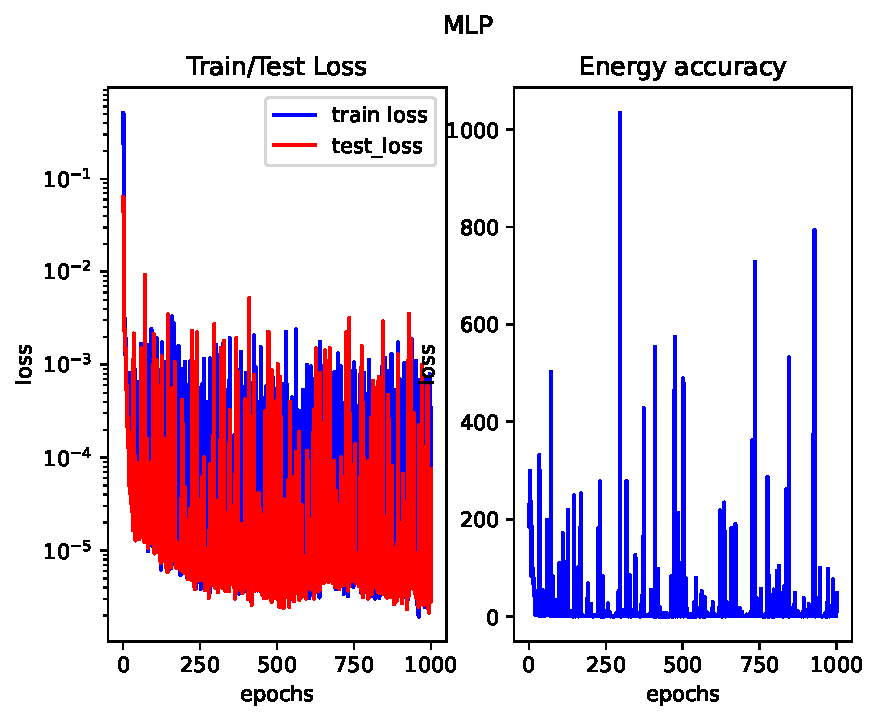
\includegraphics[width=\textwidth]{chapters/chapter5/osci_mlp_loss.pdf}
		\caption{MLP}
	\end{subfigure}
	\hfill
	\begin{subfigure}[b]{0.3\textwidth}
		\centering
		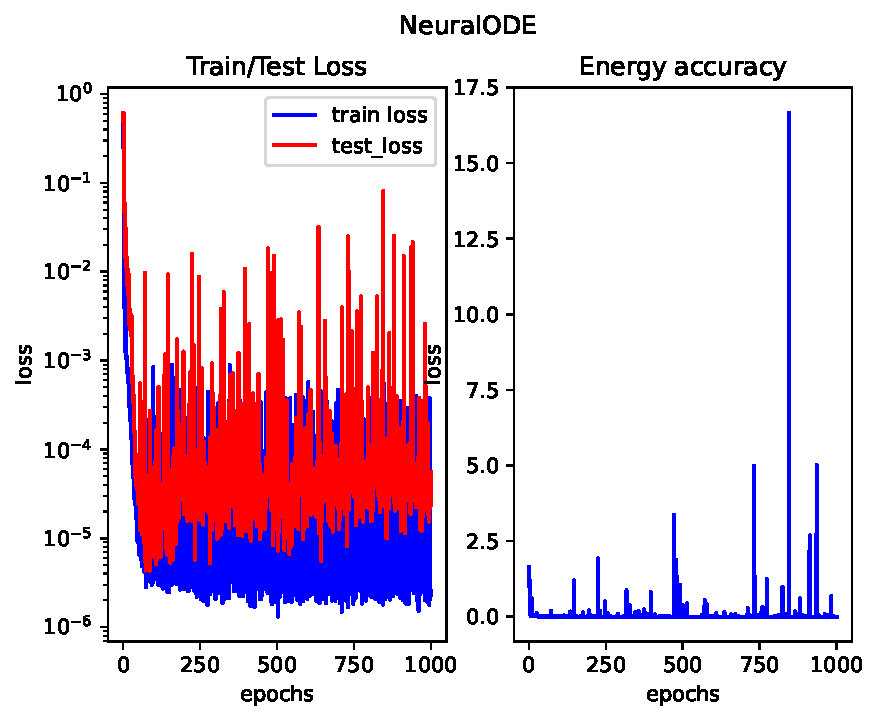
\includegraphics[width=\textwidth]{chapters/chapter5/osci_ode_loss.pdf}
		\caption{ODE}
	\end{subfigure}
	\hfill
	\begin{subfigure}[b]{0.3\textwidth}
		\centering
		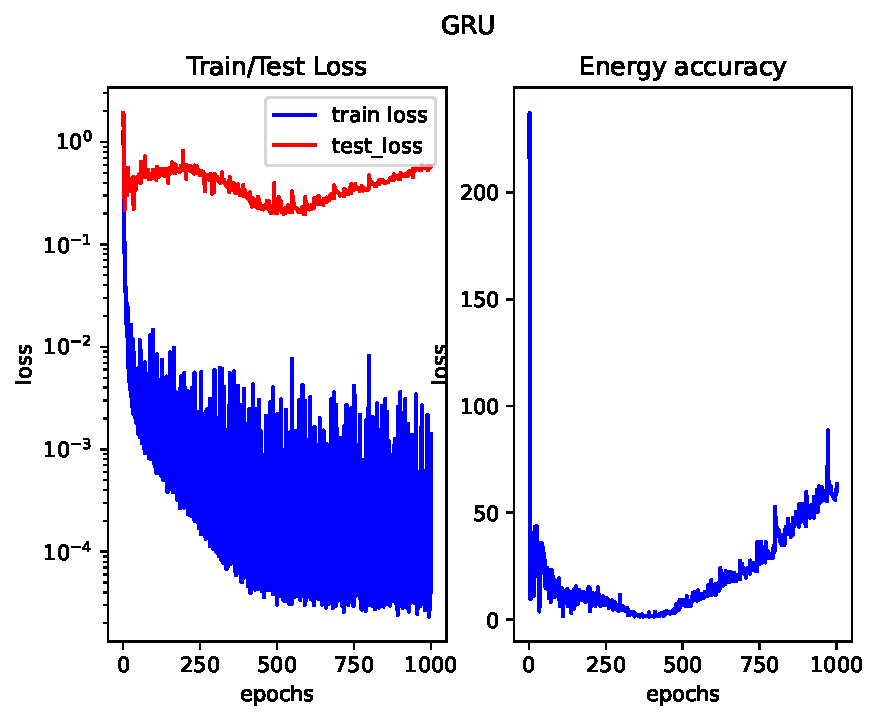
\includegraphics[width=\textwidth]{chapters/chapter5/osci_gru_loss.pdf}
		\caption{GRU}
	\end{subfigure}
	
	\vspace{0.5cm} % Adds vertical space between rows
	
	\begin{subfigure}[b]{0.3\textwidth}
		\centering
		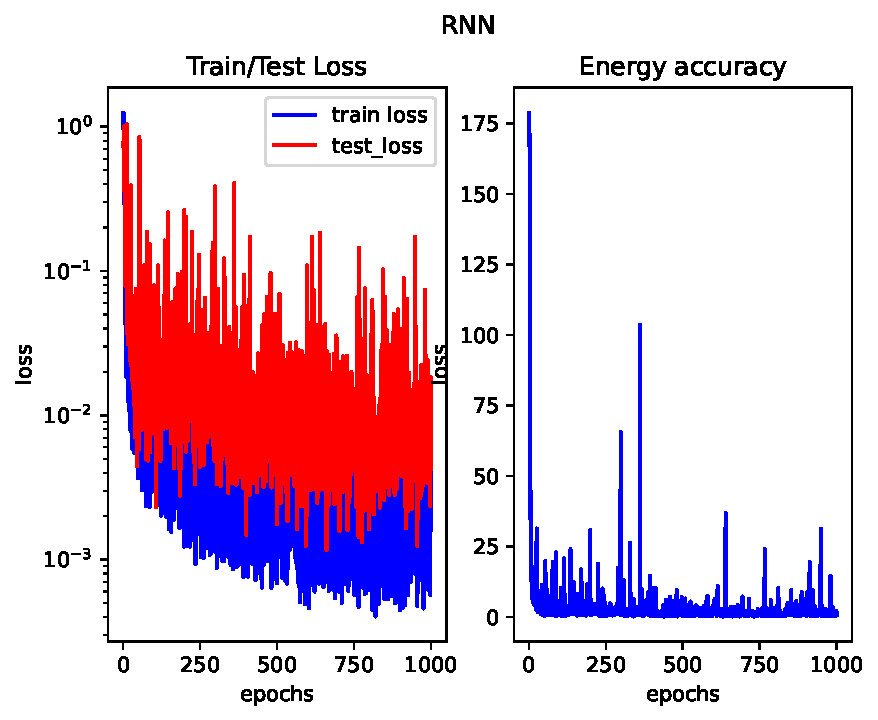
\includegraphics[width=\textwidth]{chapters/chapter5/osci_rnn_loss.pdf}
		\caption{RNN}
	\end{subfigure}
	\hfill
	\begin{subfigure}[b]{0.3\textwidth}
		\centering
		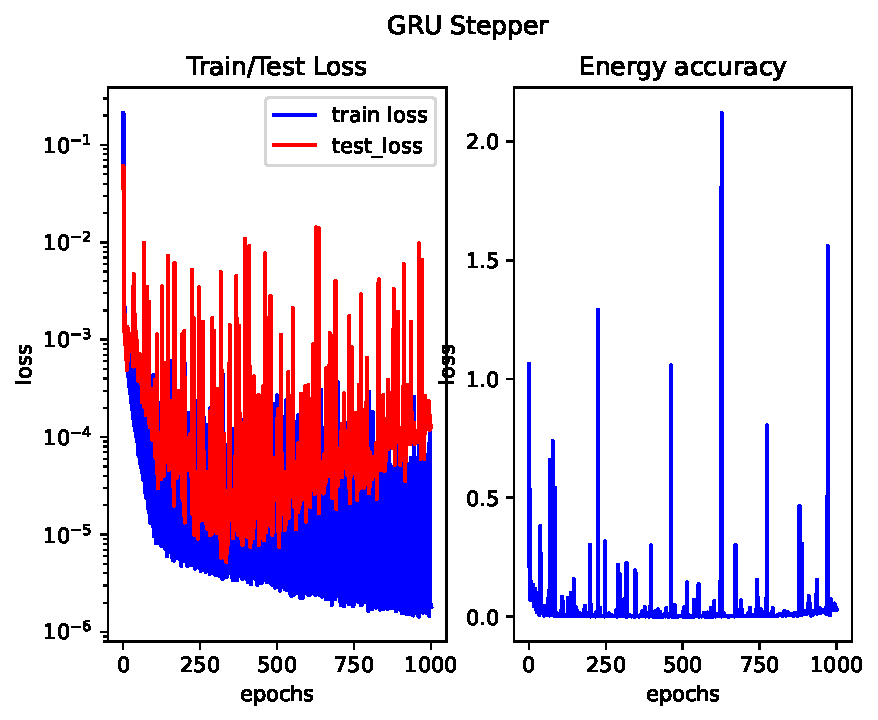
\includegraphics[width=\textwidth]{chapters/chapter5/osci_gre_loss.pdf}
		\caption{GRU Stepper}
	\end{subfigure}
	\hfill
	\begin{subfigure}[b]{0.3\textwidth}
		\centering
		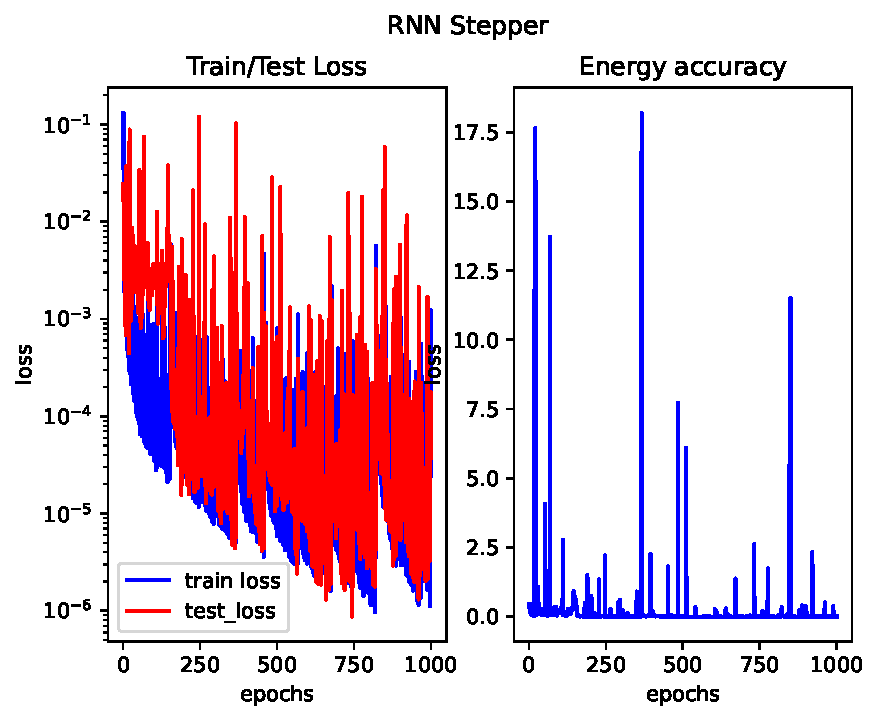
\includegraphics[width=\textwidth]{chapters/chapter5/osci_rne_loss.pdf}
		\caption{RNN stepper}
	\end{subfigure}
	
	\caption{Losses and energy accuracy on various neural models(Oscilator)}
	\label{osci_loss}
\end{figure}

\begin{figure}[H]

	\centering
	\begin{subfigure}[b]{0.3\textwidth}
		\centering
		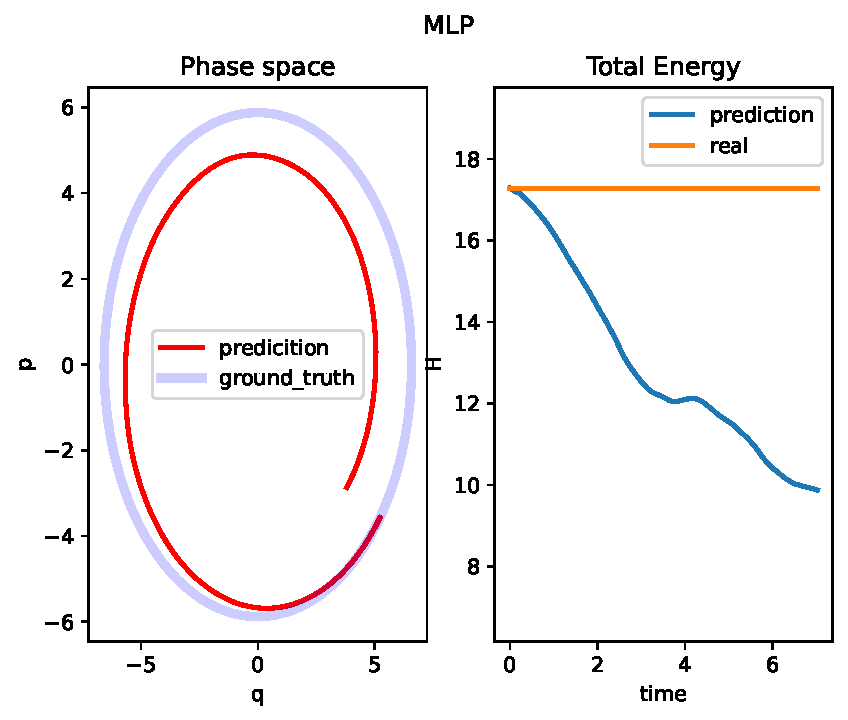
\includegraphics[width=\textwidth]{chapters/chapter5/osci_mlp_ps.pdf}
		\caption{MLP}
	\end{subfigure}
	\hfill
	\begin{subfigure}[b]{0.3\textwidth}
		\centering
		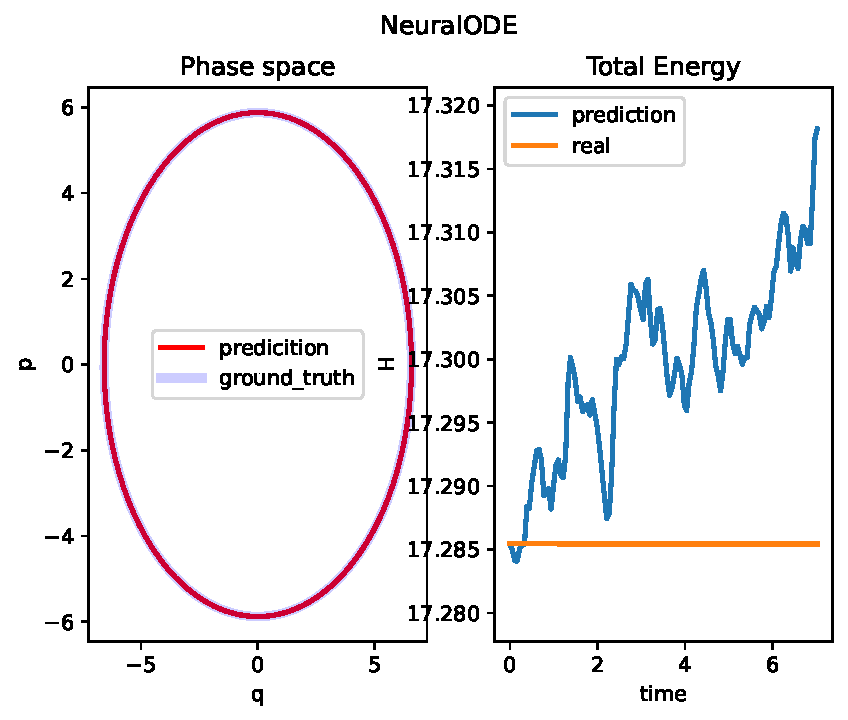
\includegraphics[width=\textwidth]{chapters/chapter5/osci_ode_ps.pdf}
		\caption{ODE}
	\end{subfigure}
	\hfill
	\begin{subfigure}[b]{0.3\textwidth}
		\centering
		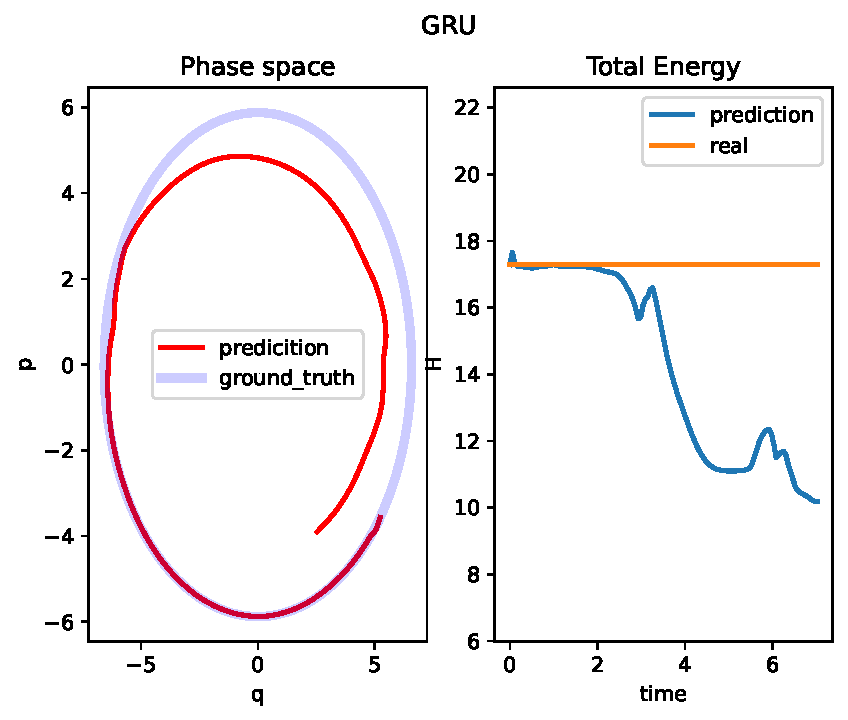
\includegraphics[width=\textwidth]{chapters/chapter5/osci_gru_ps.pdf}
		\caption{GRU}
	\end{subfigure}
	
	\vspace{0.5cm} % Adds vertical space between rows
	
	\begin{subfigure}[b]{0.3\textwidth}
		\centering
		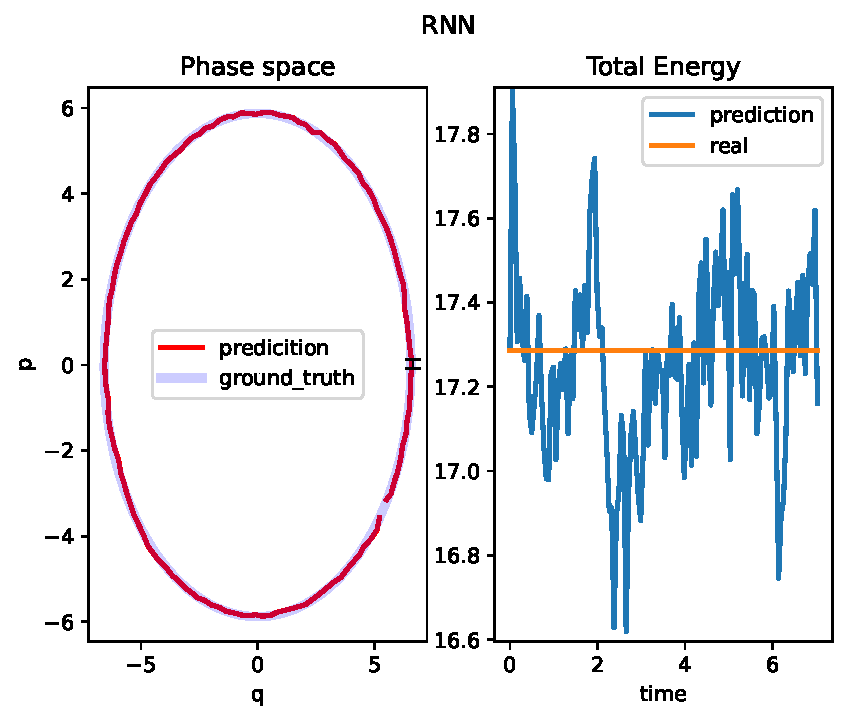
\includegraphics[width=\textwidth]{chapters/chapter5/osci_rnn_ps.pdf}
		\caption{RNN}
	\end{subfigure}
	\hfill
	\begin{subfigure}[b]{0.3\textwidth}
		\centering
		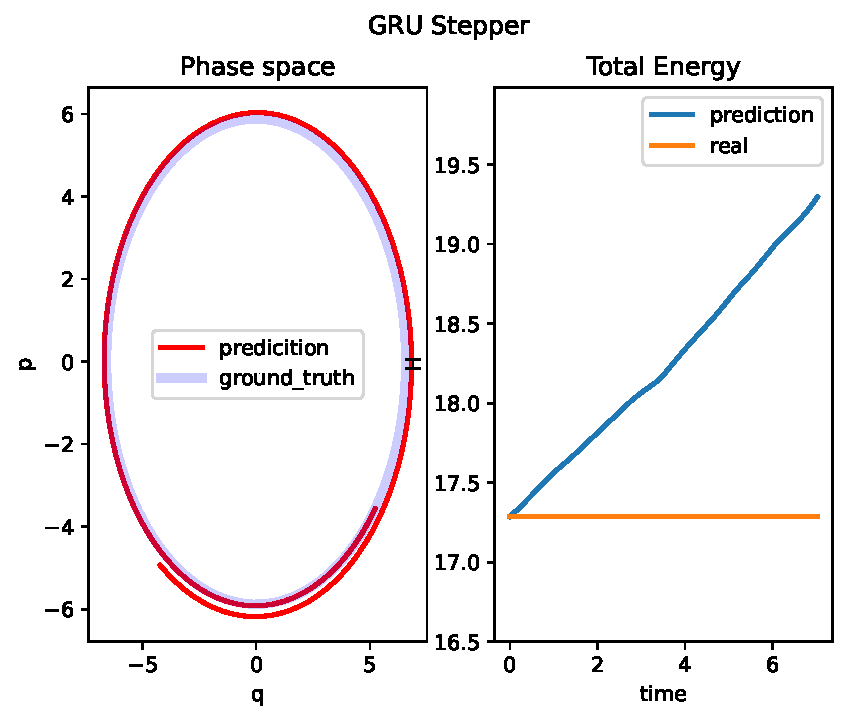
\includegraphics[width=\textwidth]{chapters/chapter5/osci_gre_ps.pdf}
		\caption{GRU Stepper}
	\end{subfigure}
	\hfill
	\begin{subfigure}[b]{0.3\textwidth}
		\centering
		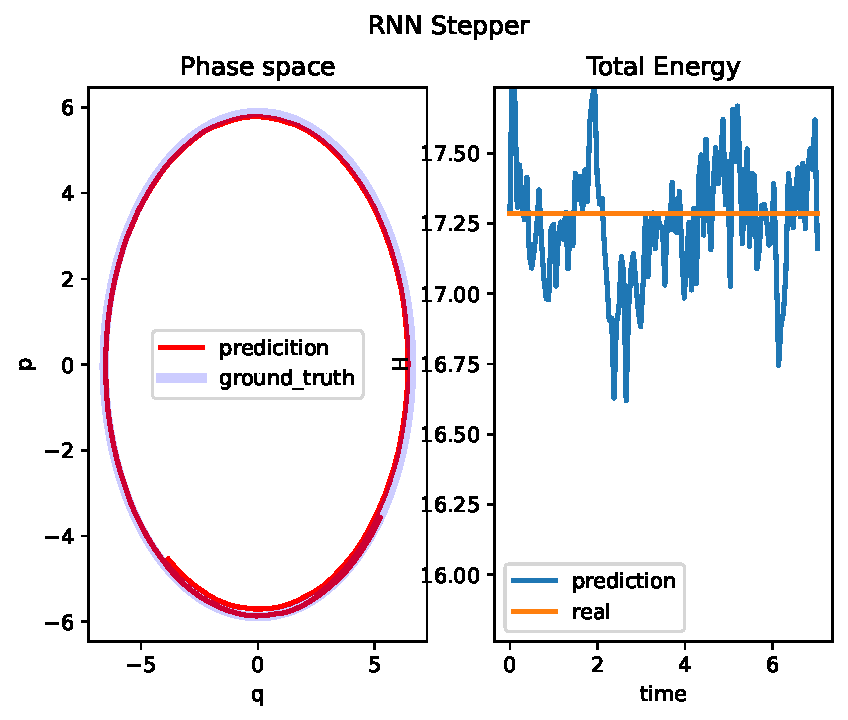
\includegraphics[width=\textwidth]{chapters/chapter5/osci_rne_ps.pdf}
		\caption{RNN stepper}
	\end{subfigure}
	
	\caption{Evaluation of the sample on the models, Trajectory and Energy(Oscilator)}
	\label{osci_traj}
\end{figure}
	

 

\subsection{Twobody-problem}
In previous chapter we disscused about creation of the Twobody Dataset.
In this Experiment we chose masses $m=\{1.0,3.0\}$ and $G=1$, we made 30 trajectories for training data and 3 trajectories for test data with 128 time points in one period.\\
The train data is batched an we have done batched leraning\begin{equation}
	\dot{\mathbf{x}} = \mathbf{A}(||\mathbf{q_1(t=0)}||)\mathbf{x},\text{  }\mathbf{x} = \begin{bmatrix}
		\mathbf{q}\\
		\mathbf{p}
	\end{bmatrix}
\end{equation} The matrix $\mathbf{A}$ is constant only for dynamics of one trajectory.\\
We train the models with "rollout" technique, exactly like explained in the oscilator case and we got following results \ref{body2_loss}, \ref{body2_traj}, \ref{body2_ps}.
\begin{itemize}
	\item Multilayer perceptron\\
	From the loss figure we see that the model has learned a hamiltonian system. Even the energy accuracy looks very stable. On the other hand the evaluation plot is little bit inaccurate.
	
	
	\item NeuralODE\\
	The trajectory is accurate and energy at evaluation sample looks that hold conservative property. Over all it is most accurate model of all.
	
	
	\item GRU\\
	similar to MLP the trajectory is little bit inaccurate but the energy shows conservative property.
	
	\item RNN\\
	It looks similar to GRU but the trajectory looks like it osclates around ground truth data 

	\item GRU Time Stepper\\
	The trajectory and energy on the evaluation sample looks inaccurate but it follows the flow of trajectory. ´

	\item RNN Time Stepper\\
	It has same characteristics as GRU Stepper but it has slightly worse perforamnce,
	
\end{itemize}

\begin{figure}[H]
	\centering
	\begin{subfigure}[b]{0.3\textwidth}
		\centering
		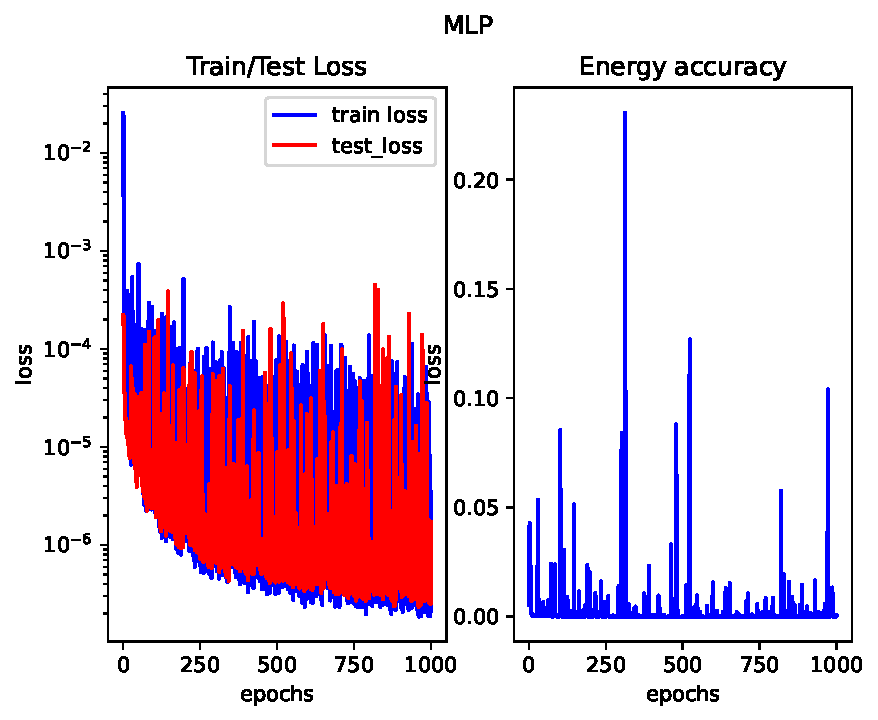
\includegraphics[width=\textwidth]{chapters/chapter5/body2_mlp_loss.pdf}
		\caption{MLP}
	\end{subfigure}
	\hfill
	\begin{subfigure}[b]{0.3\textwidth}
		\centering
		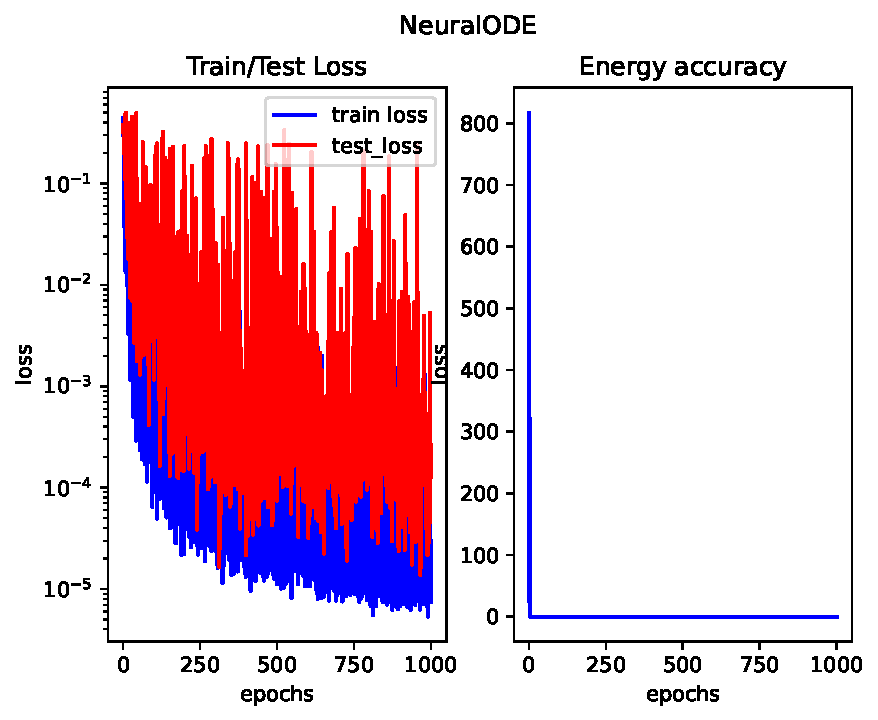
\includegraphics[width=\textwidth]{chapters/chapter5/body2_ode_loss.pdf}
		\caption{ODE}
	\end{subfigure}
	\hfill
	\begin{subfigure}[b]{0.3\textwidth}
		\centering
		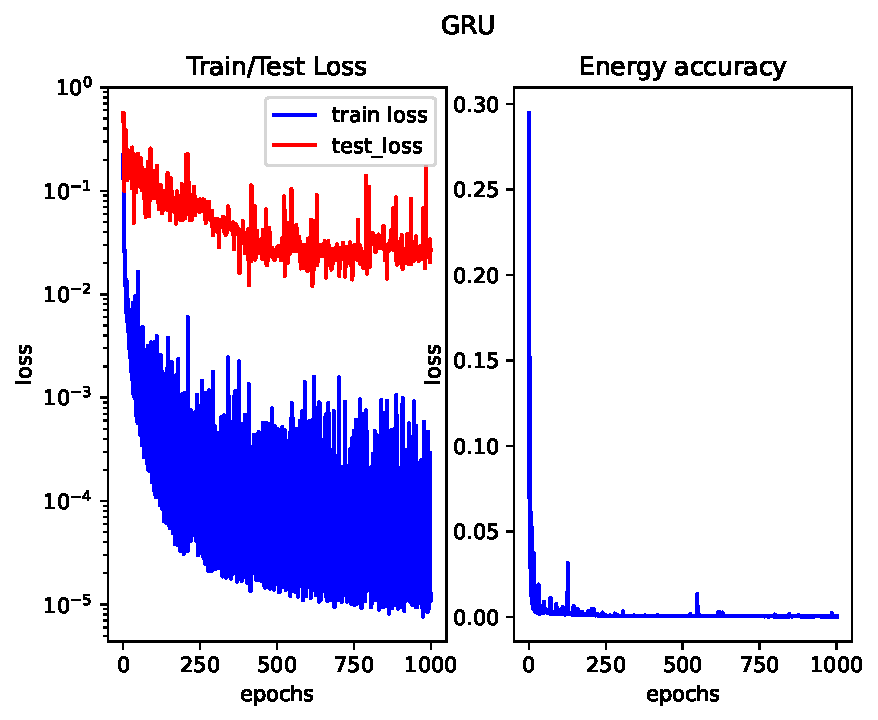
\includegraphics[width=\textwidth]{chapters/chapter5/body2_gru_loss.pdf}
		\caption{GRU}
	\end{subfigure}
	
	\vspace{0.5cm} % Adds vertical space between rows
	
	\begin{subfigure}[b]{0.3\textwidth}
		\centering
		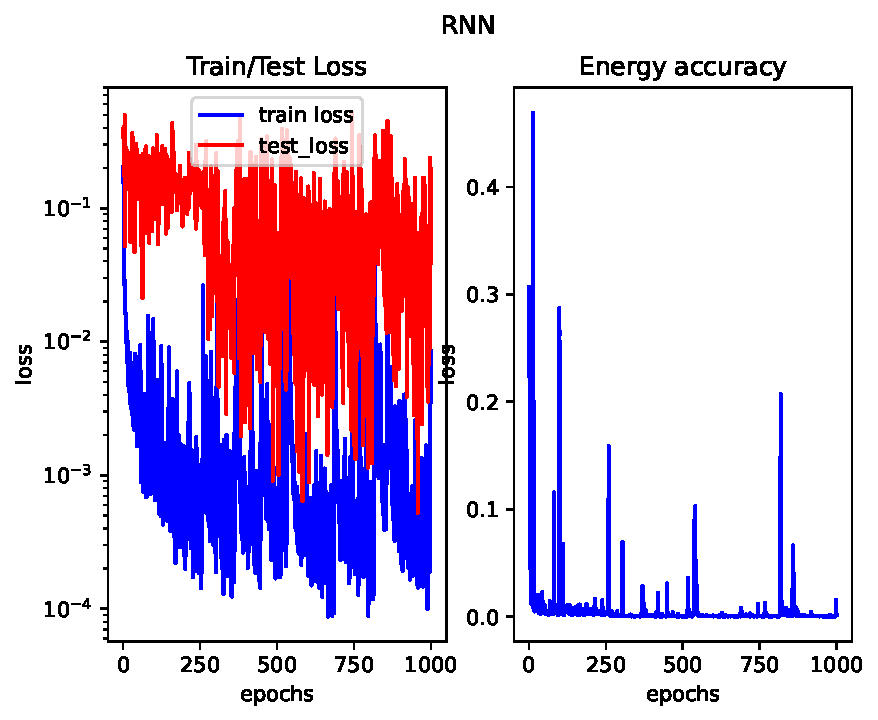
\includegraphics[width=\textwidth]{chapters/chapter5/body2_rnn_loss.pdf}
		\caption{RNN}
	\end{subfigure}
	\hfill
	\begin{subfigure}[b]{0.3\textwidth}
		\centering
		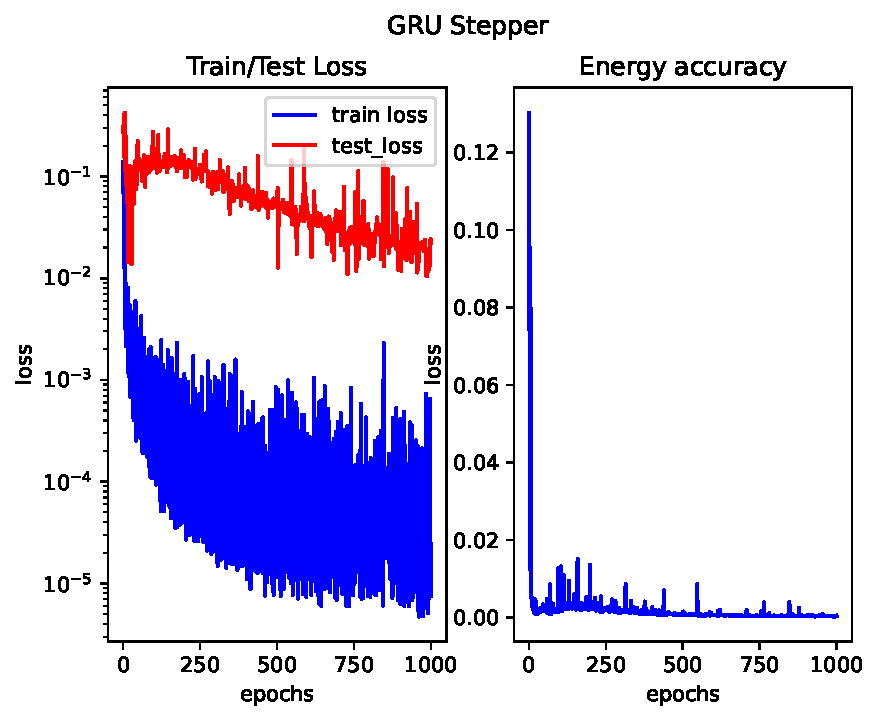
\includegraphics[width=\textwidth]{chapters/chapter5/body2_gre_loss.pdf}
		\caption{GRU Stepper}
	\end{subfigure}
	\hfill
	\begin{subfigure}[b]{0.3\textwidth}
		\centering
		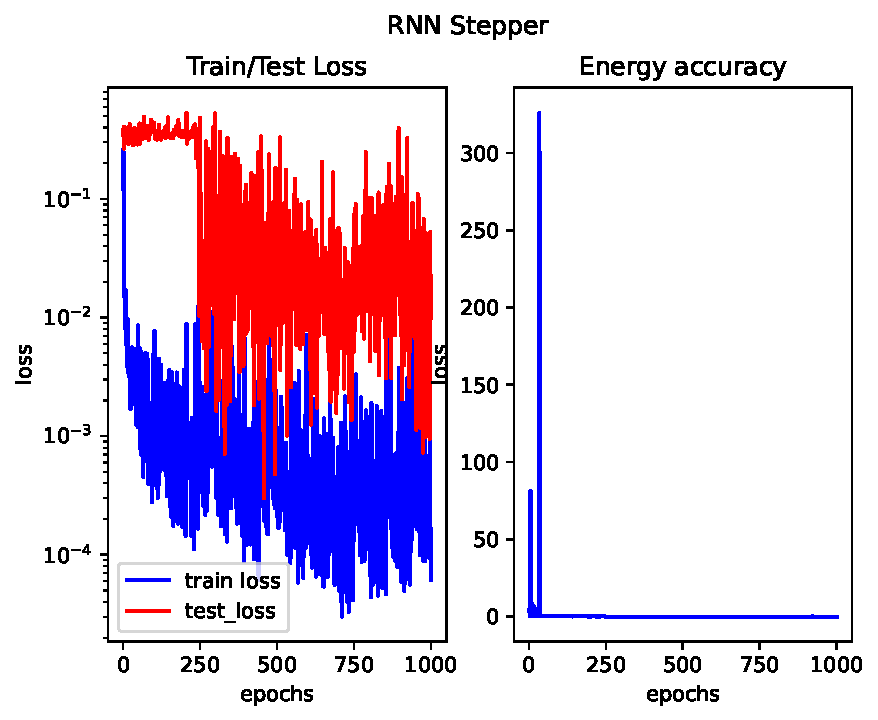
\includegraphics[width=\textwidth]{chapters/chapter5/body2_rne_loss.pdf}
		\caption{RNN stepper}
	\end{subfigure}
	
	\caption{Losses and energy accuracy on various neural models(Oscilator)}
	\label{body2_loss}
\end{figure}

\begin{figure}[H]
	\centering
	\begin{subfigure}[b]{0.3\textwidth}
		\centering
		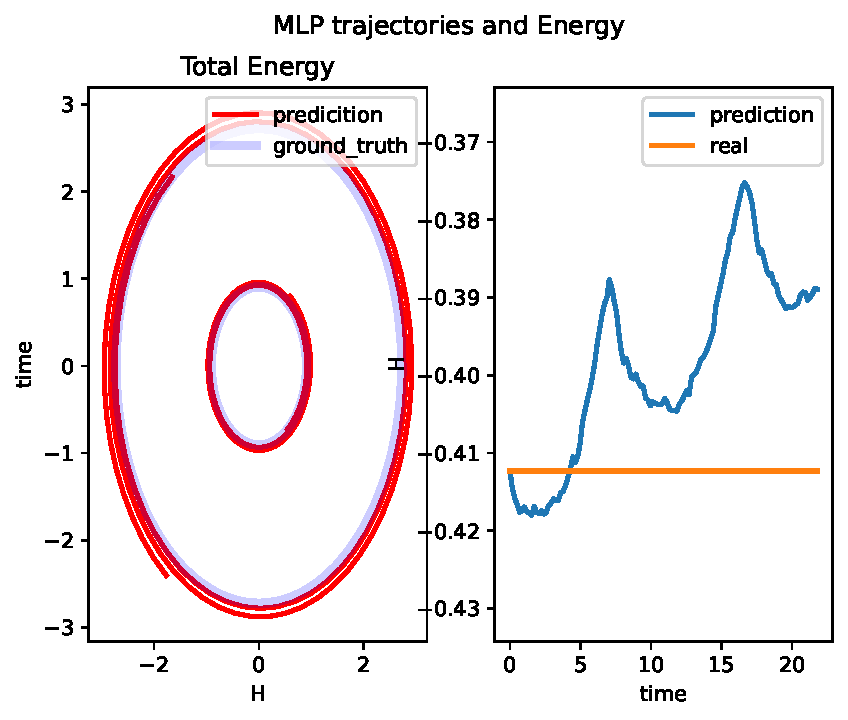
\includegraphics[width=\textwidth]{chapters/chapter5/body2_mlp_traj.pdf}
		\caption{MLP}
	\end{subfigure}
	\hfill
	\begin{subfigure}[b]{0.3\textwidth}
		\centering
		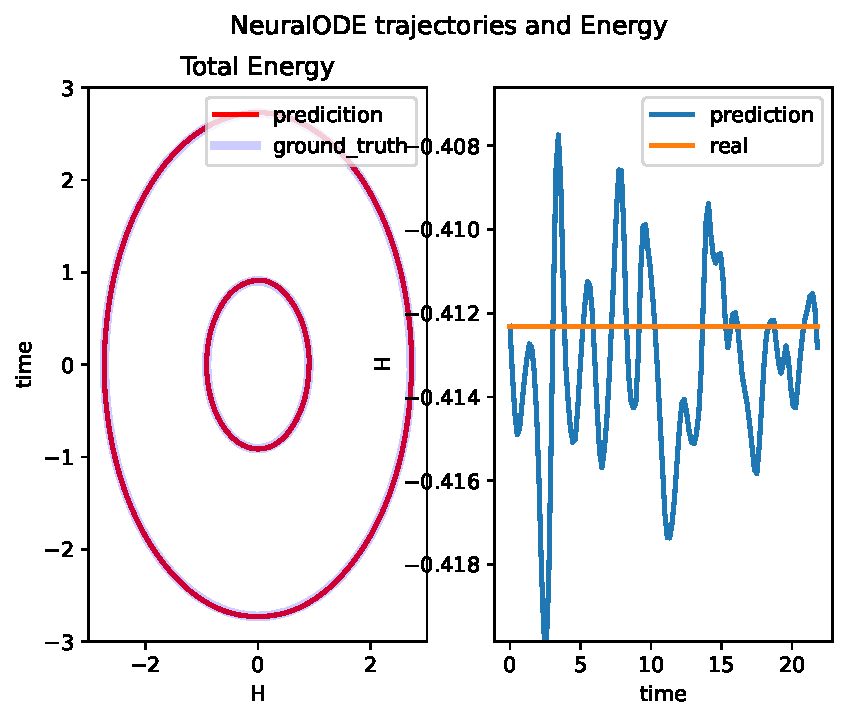
\includegraphics[width=\textwidth]{chapters/chapter5/body2_ode_traj.pdf}
		\caption{ODE}
	\end{subfigure}
	\hfill
	\begin{subfigure}[b]{0.3\textwidth}
		\centering
		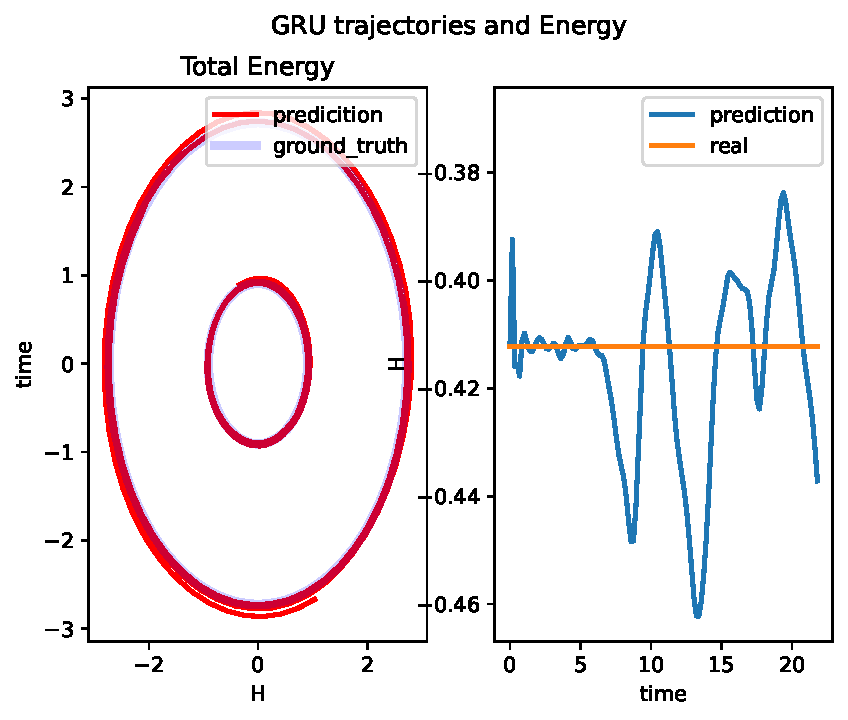
\includegraphics[width=\textwidth]{chapters/chapter5/body2_gru_traj.pdf}
		\caption{GRU}
	\end{subfigure}
	
	\vspace{0.5cm} % Adds vertical space between rows
	
	\begin{subfigure}[b]{0.3\textwidth}
		\centering
		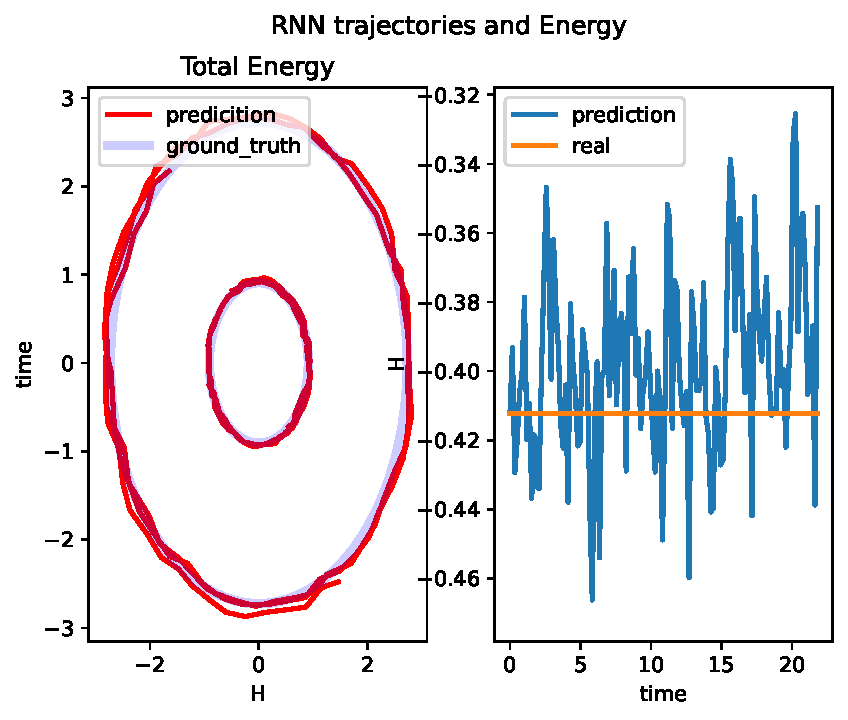
\includegraphics[width=\textwidth]{chapters/chapter5/body2_rnn_traj.pdf}
		\caption{RNN}
	\end{subfigure}
	\hfill
	\begin{subfigure}[b]{0.3\textwidth}
		\centering
		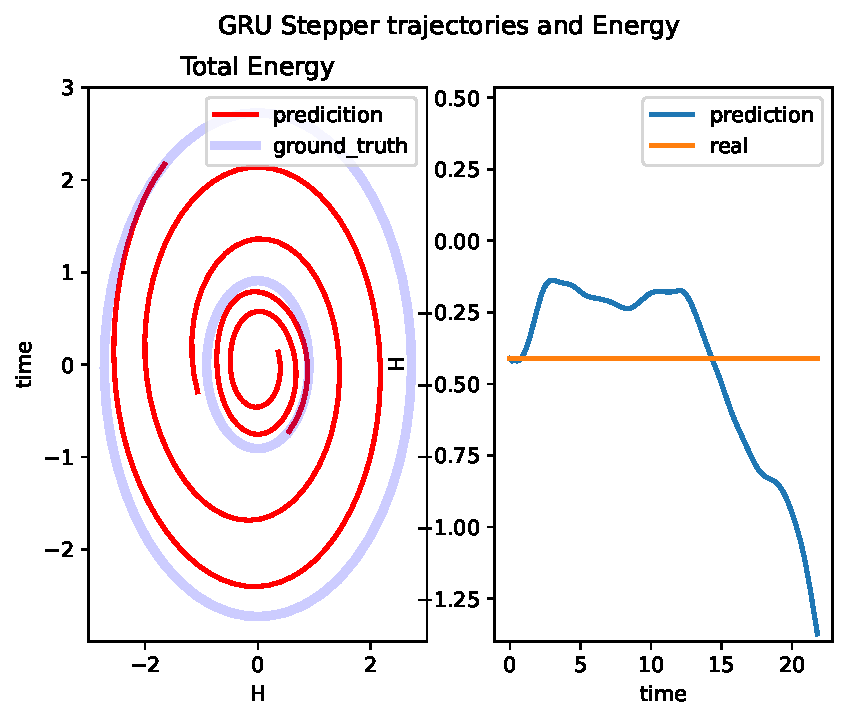
\includegraphics[width=\textwidth]{chapters/chapter5/body2_gre_traj.pdf}
		\caption{GRU Stepper}
	\end{subfigure}
	\hfill
	\begin{subfigure}[b]{0.3\textwidth}
		\centering
		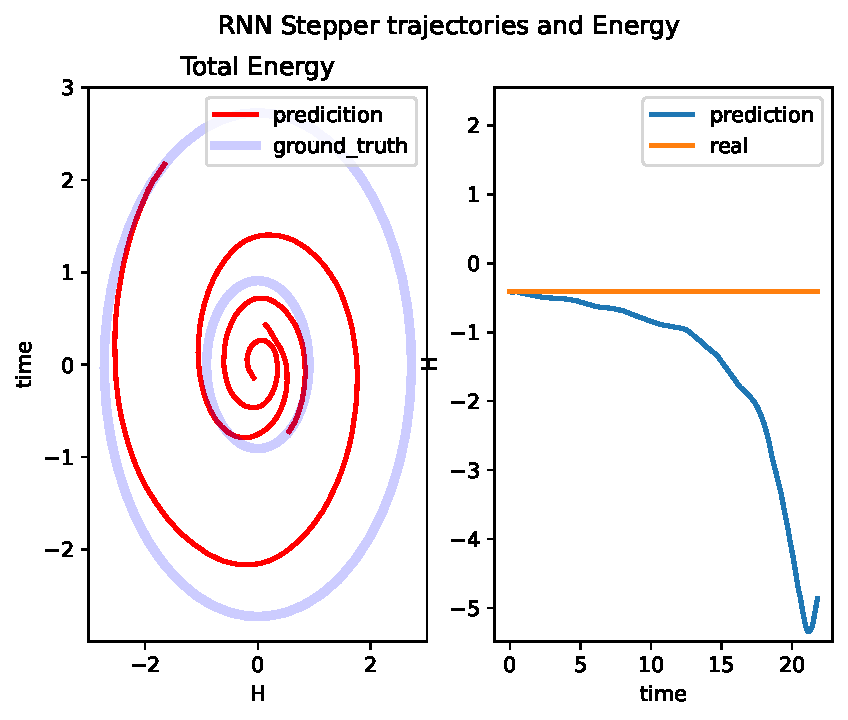
\includegraphics[width=\textwidth]{chapters/chapter5/body2_rne_traj.pdf}
		\caption{RNN stepper}
	\end{subfigure}
	
	\caption{Evaluation of the sample on the models, Trajectory and Energy(Twobody)}
	\label{body2_traj}
\end{figure}

\begin{figure}[H]
	\centering
	\begin{subfigure}[b]{0.3\textwidth}
		\centering
		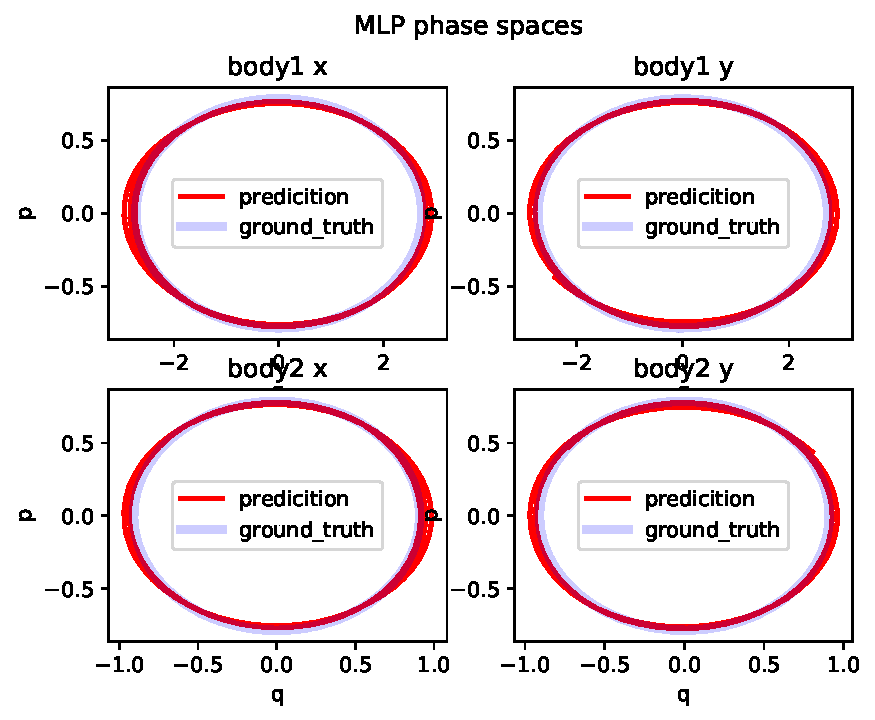
\includegraphics[width=\textwidth]{chapters/chapter5/body2_mlp_ps.pdf}
		\caption{MLP}
	\end{subfigure}
	\hfill
	\begin{subfigure}[b]{0.3\textwidth}
		\centering
		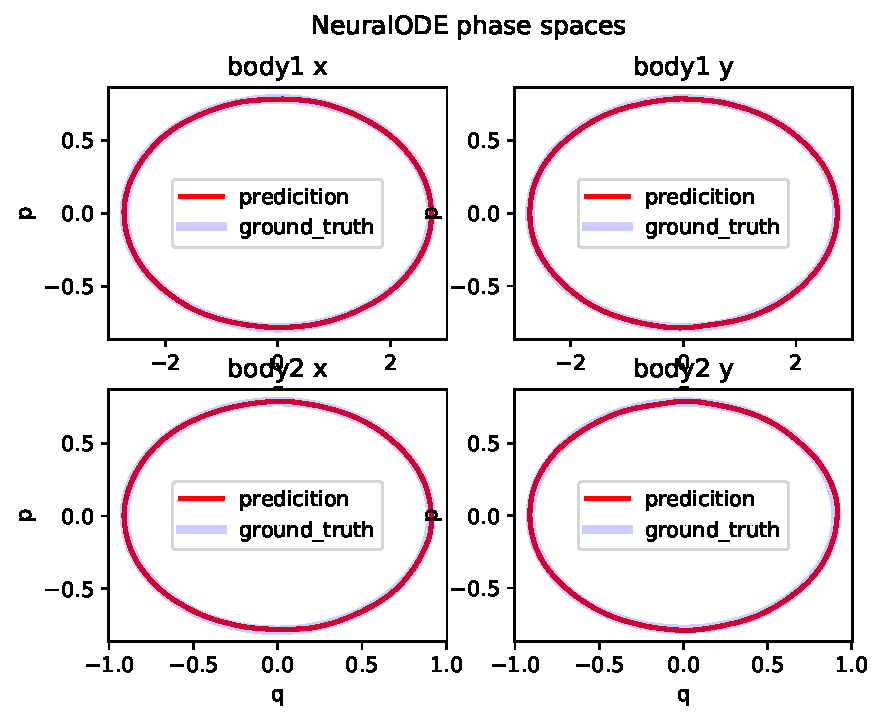
\includegraphics[width=\textwidth]{chapters/chapter5/body2_ode_ps.pdf}
		\caption{ODE}
	\end{subfigure}
	\hfill
	\begin{subfigure}[b]{0.3\textwidth}
		\centering
		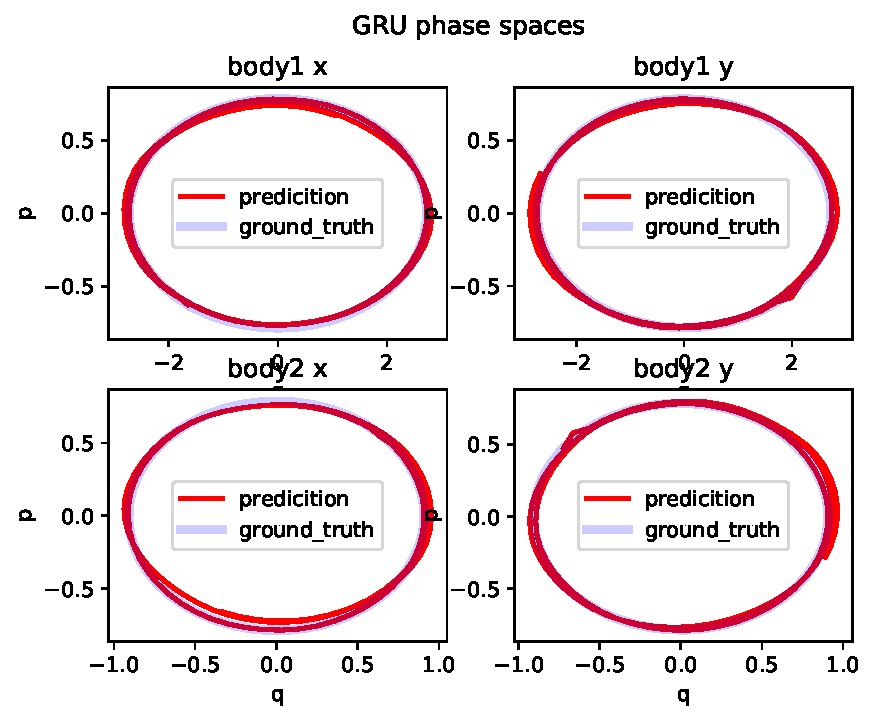
\includegraphics[width=\textwidth]{chapters/chapter5/body2_gru_ps.pdf}
		\caption{GRU}
	\end{subfigure}
	
	\vspace{0.5cm} % Adds vertical space between rows
	
	\begin{subfigure}[b]{0.3\textwidth}
		\centering
		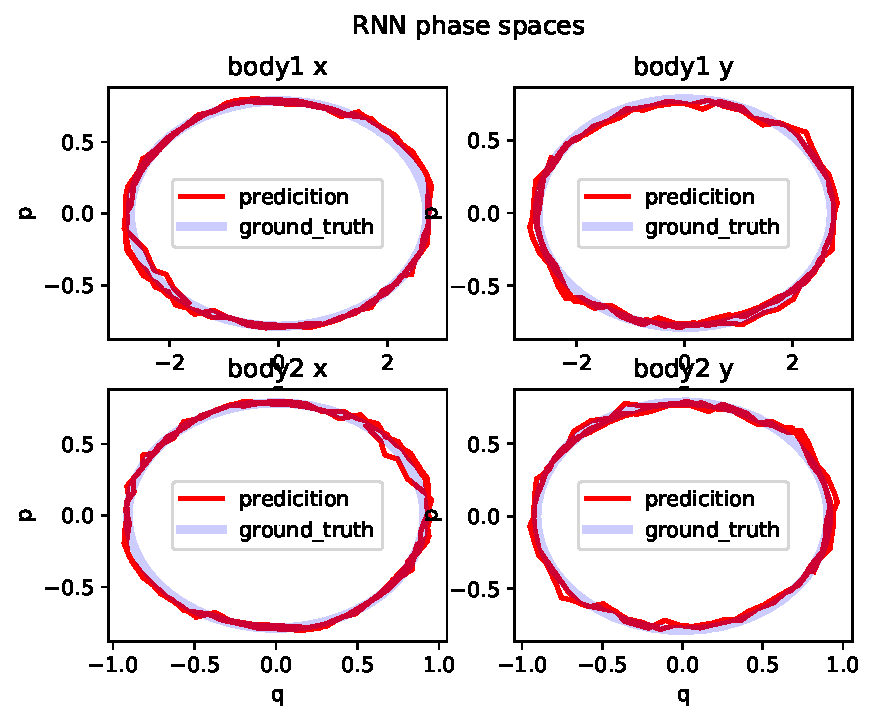
\includegraphics[width=\textwidth]{chapters/chapter5/body2_rnn_ps.pdf}
		\caption{RNN}
	\end{subfigure}
	\hfill
	\begin{subfigure}[b]{0.3\textwidth}
		\centering
		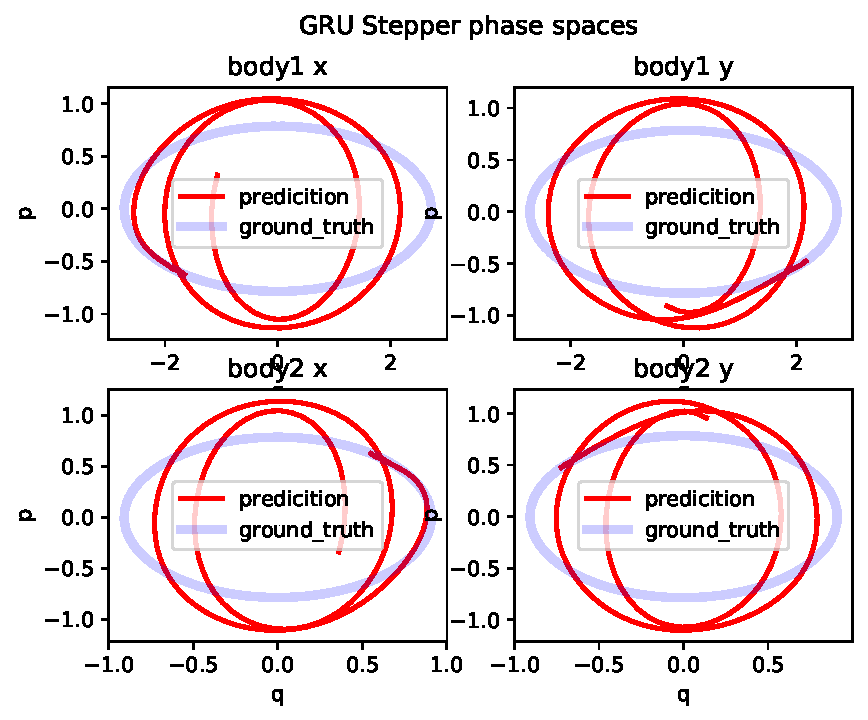
\includegraphics[width=\textwidth]{chapters/chapter5/body2_gre_ps.pdf}
		\caption{GRU Stepper}
	\end{subfigure}
	\hfill
	\begin{subfigure}[b]{0.3\textwidth}
		\centering
		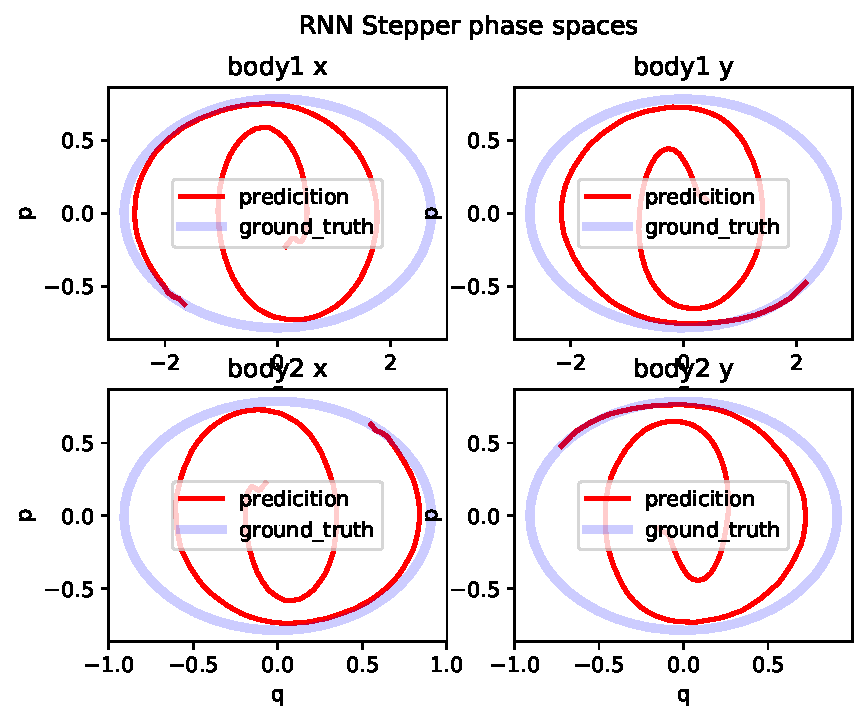
\includegraphics[width=\textwidth]{chapters/chapter5/body2_rne_ps.pdf}
		\caption{RNN stepper}
	\end{subfigure}
	
	\caption{Evaluation of the sample on the models, phase space (Twobody)}
	\label{body2_ps}
\end{figure}



\subsection{Three-body problem}
In previous chapter we discussed about creation of the Three-body Dataset.
In this Experiment we chose masses $m=\{1.0,1.0,1.0\}$ and $G=1$, we made 30 trajectories for training data and 3 trajectories for test data with 128 time points in one period.\\
The trajectories are different because we set $\alpha\in[0,1.0 \text{rad}]$ as a rotation around the origin. In this case we have same Total Energy for all trajectories\\ \begin{equation}
	\dot{\mathbf{x}} = \mathbf{A}(\mathbf{q})\mathbf{x},\text{  }\mathbf{x} = \begin{bmatrix}
		\mathbf{q}\\
		\mathbf{p}
	\end{bmatrix}
\end{equation} The matrix $\mathbf{A}$ is variational and depends strictly on position of the body in every timestep.
We used batched technique to learn the dataset and we got following results in Figures \ref{body3_loss}, \ref{body3_traj}, \ref{body3_ps}
\begin{itemize}
	\item Multilayer perceptron\\
	It trained well, Energy accuracy has gone minmal after 150 epochs of training and shows very good trajectory.

	
	\item NeuralODE\\
	Interestingly enough the trajectory on evaluation sample looks accurate but total energy doesn't look accurate. Energy accuarcy metric is after 200 epoch minimal which is good sign.´   ´

	\item GRU\\
	The model looks overtrained if we look at loss figure. Furthermore trajectory and Energy is inaccurate, but it follows the figure 8 shape. 

	\item RNN\\
	This model has failed.

	\item GRU Time Stepper\\
	It shows very good performance, similary to Neural ODE. 

	\item RNN Time Stepper\\
	It looks better then RNN but it looks like it has issues to learn for data.

\end{itemize}
From all Datasets we can conclude that RNN and RNN Stepper are bad models for the physics problems. On the other hand RNN model shows little bit of good performance but it isn't right model for this task. Through experimentations we see that NeuralODE and GRU Stepper show better performance then the baseline MLP.
\begin{figure}[H]
	\centering
	\begin{subfigure}[b]{0.3\textwidth}
		\centering
		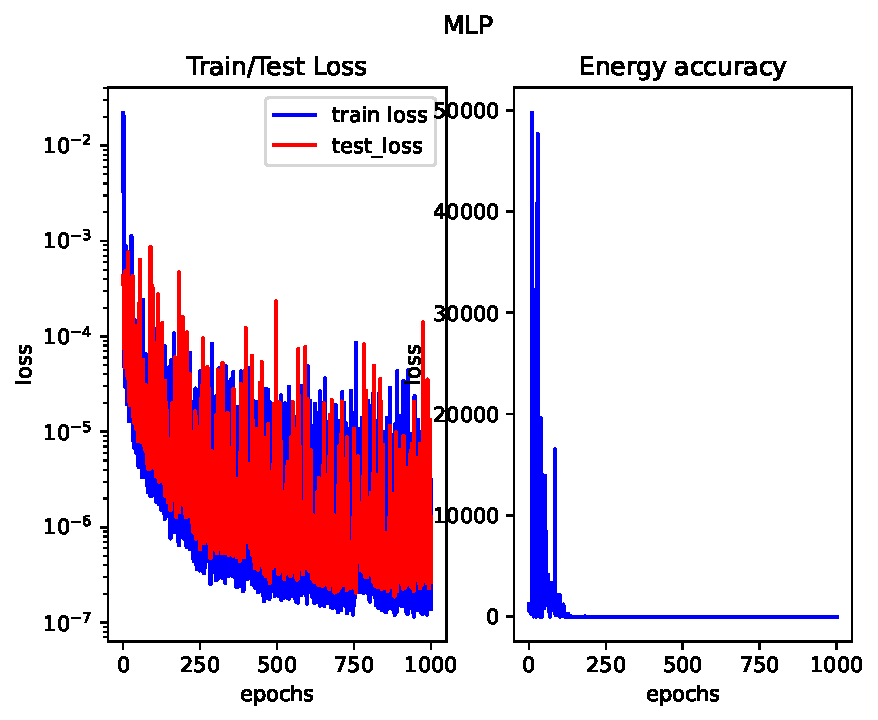
\includegraphics[width=\textwidth]{chapters/chapter5/body3_mlp_loss.pdf}
		\caption{MLP}
	\end{subfigure}
	\hfill
	\begin{subfigure}[b]{0.3\textwidth}
		\centering
		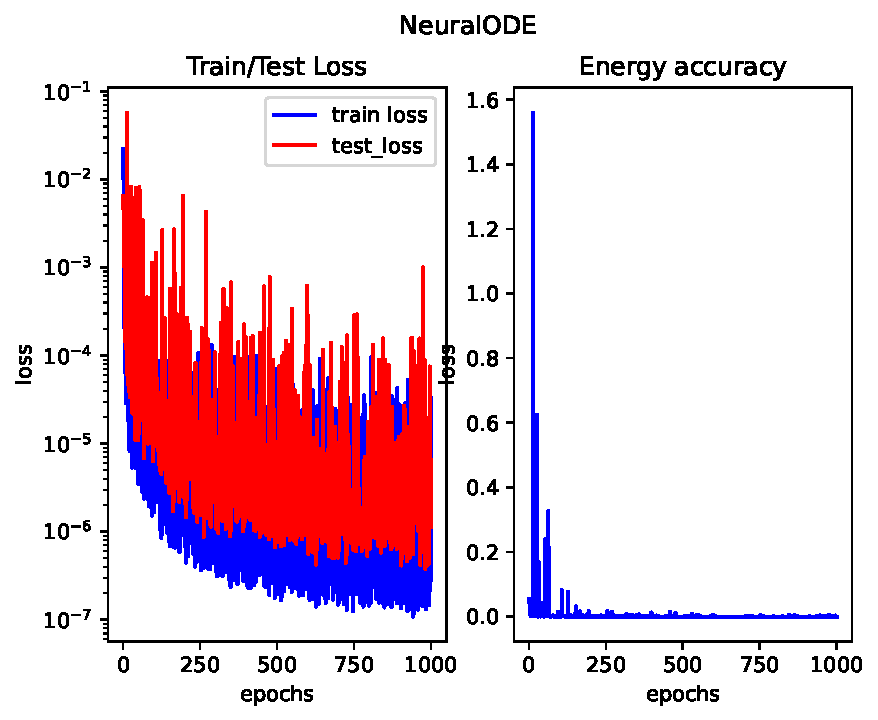
\includegraphics[width=\textwidth]{chapters/chapter5/body3_ode_loss.pdf}
		\caption{ODE}
	\end{subfigure}
	\hfill
	\begin{subfigure}[b]{0.3\textwidth}
		\centering
		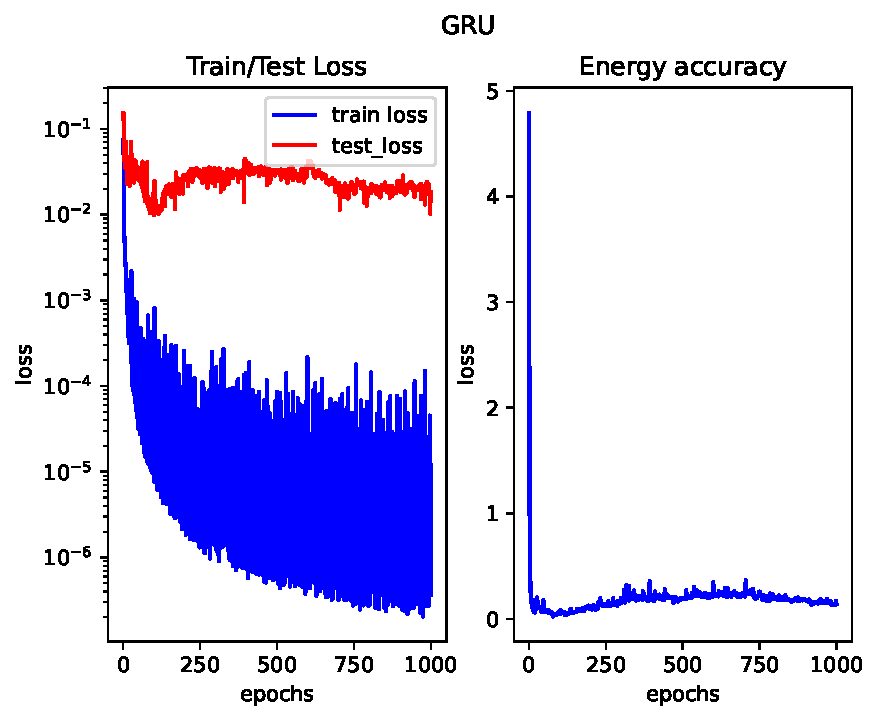
\includegraphics[width=\textwidth]{chapters/chapter5/body3_gru_loss.pdf}
		\caption{GRU}
	\end{subfigure}
	
	\vspace{0.5cm} % Adds vertical space between rows
	
	\begin{subfigure}[b]{0.3\textwidth}
		\centering
		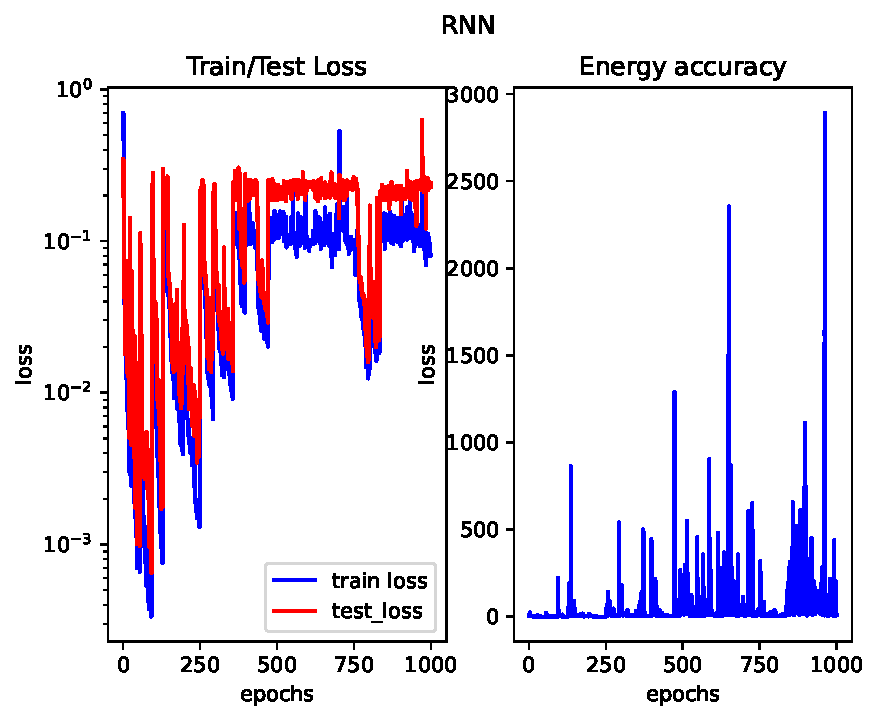
\includegraphics[width=\textwidth]{chapters/chapter5/body3_rnn_loss.pdf}
		\caption{RNN}
	\end{subfigure}
	\hfill
	\begin{subfigure}[b]{0.3\textwidth}
		\centering
		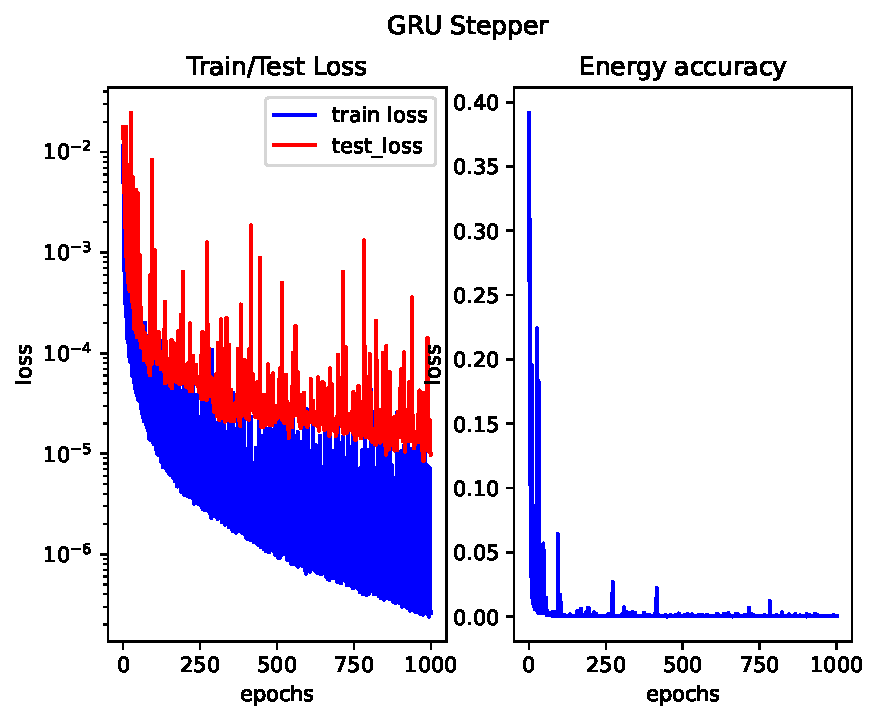
\includegraphics[width=\textwidth]{chapters/chapter5/body3_gre_loss.pdf}
		\caption{GRU Stepper}
	\end{subfigure}
	\hfill
	\begin{subfigure}[b]{0.3\textwidth}
		\centering
		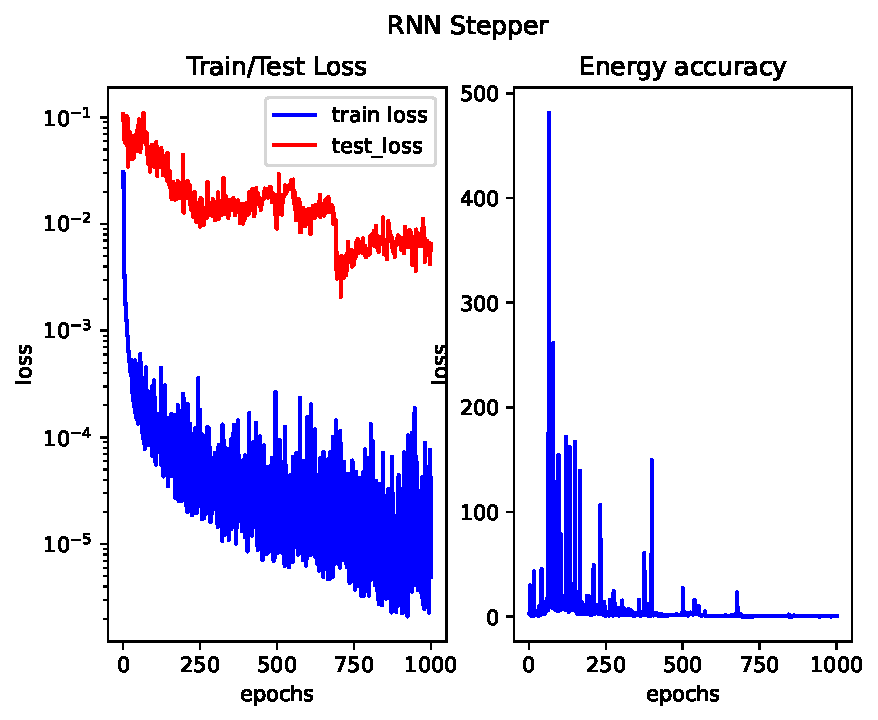
\includegraphics[width=\textwidth]{chapters/chapter5/body3_rne_loss.pdf}
		\caption{RNN stepper}
	\end{subfigure}
	
	\caption{Losses and energy accuracy on various neural models(Threebody)}
	\label{body3_loss}
\end{figure}

\begin{figure}[H]
	\centering
	\begin{subfigure}[b]{0.3\textwidth}
		\centering
		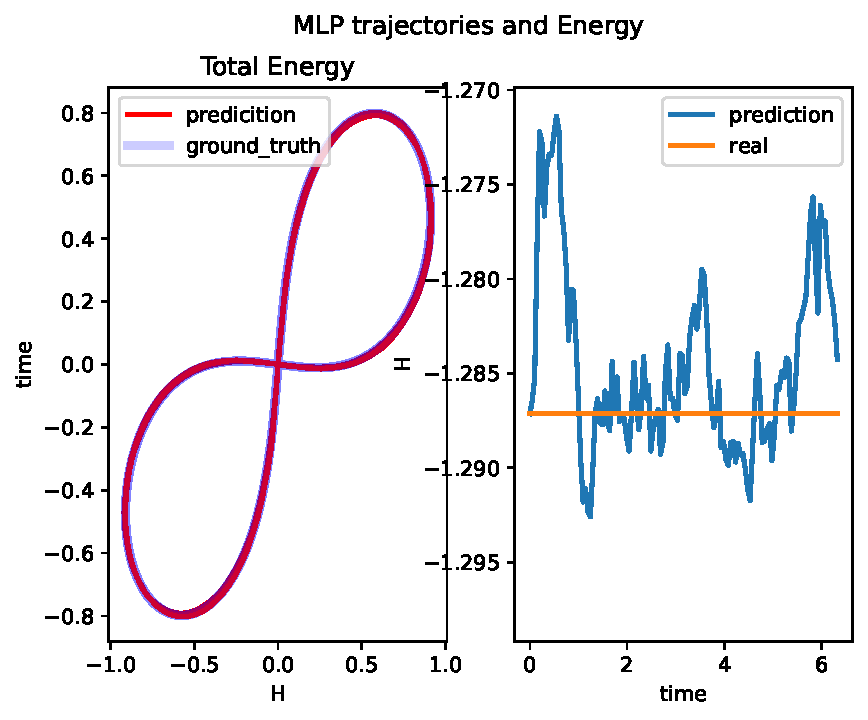
\includegraphics[width=\textwidth]{chapters/chapter5/body3_mlp_traj.pdf}
		\caption{MLP}
	\end{subfigure}
	\hfill
	\begin{subfigure}[b]{0.3\textwidth}
		\centering
		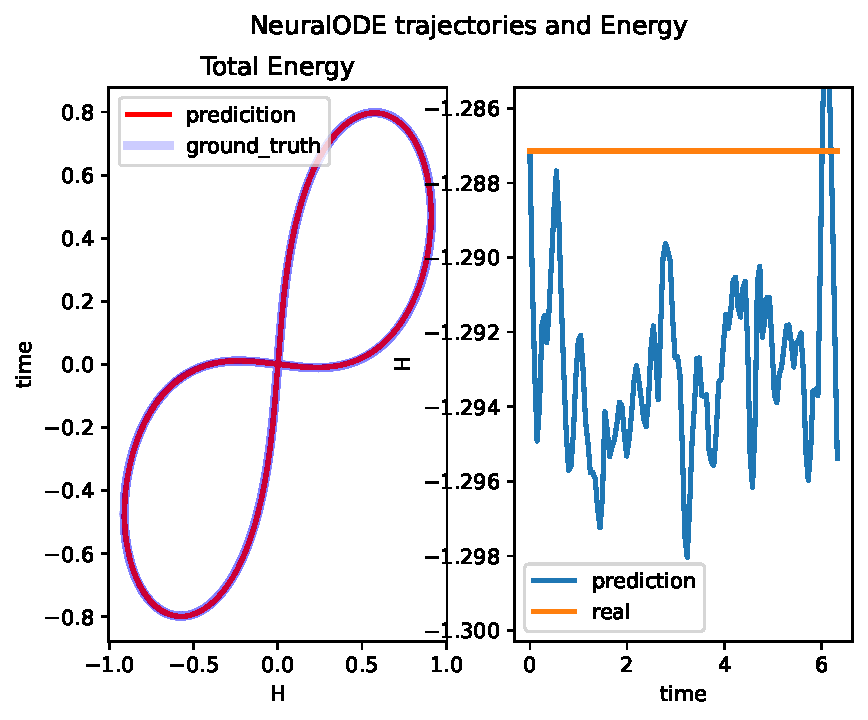
\includegraphics[width=\textwidth]{chapters/chapter5/body3_ode_traj.pdf}
		\caption{ODE}
	\end{subfigure}
	\hfill
	\begin{subfigure}[b]{0.3\textwidth}
		\centering
		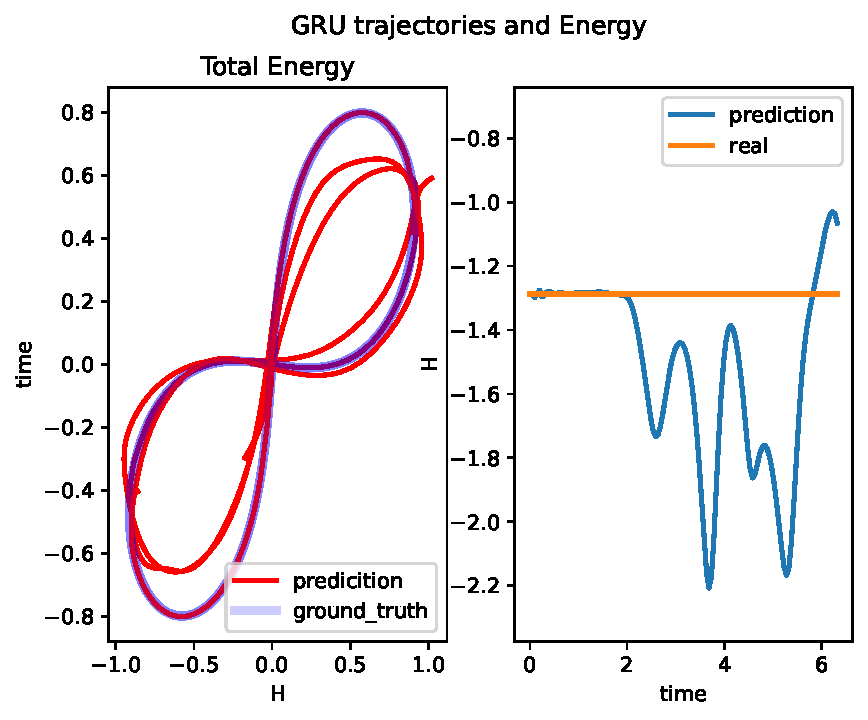
\includegraphics[width=\textwidth]{chapters/chapter5/body3_gru_traj.pdf}
		\caption{GRU}
	\end{subfigure}
	
	\vspace{0.5cm} % Adds vertical space between rows
	
	\begin{subfigure}[b]{0.3\textwidth}
		\centering
		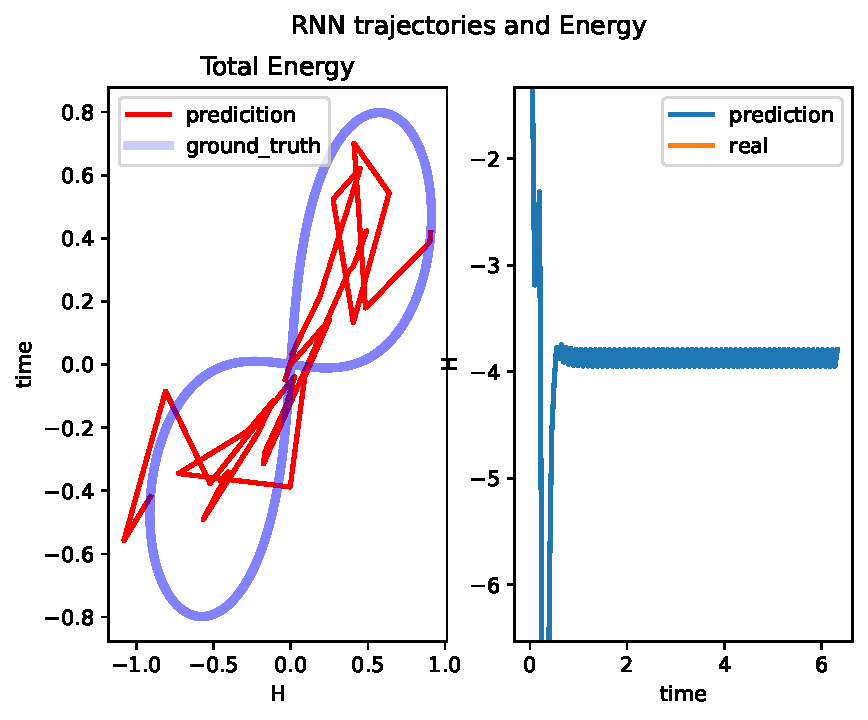
\includegraphics[width=\textwidth]{chapters/chapter5/body3_rnn_traj.pdf}
		\caption{RNN}
	\end{subfigure}
	\hfill
	\begin{subfigure}[b]{0.3\textwidth}
		\centering
		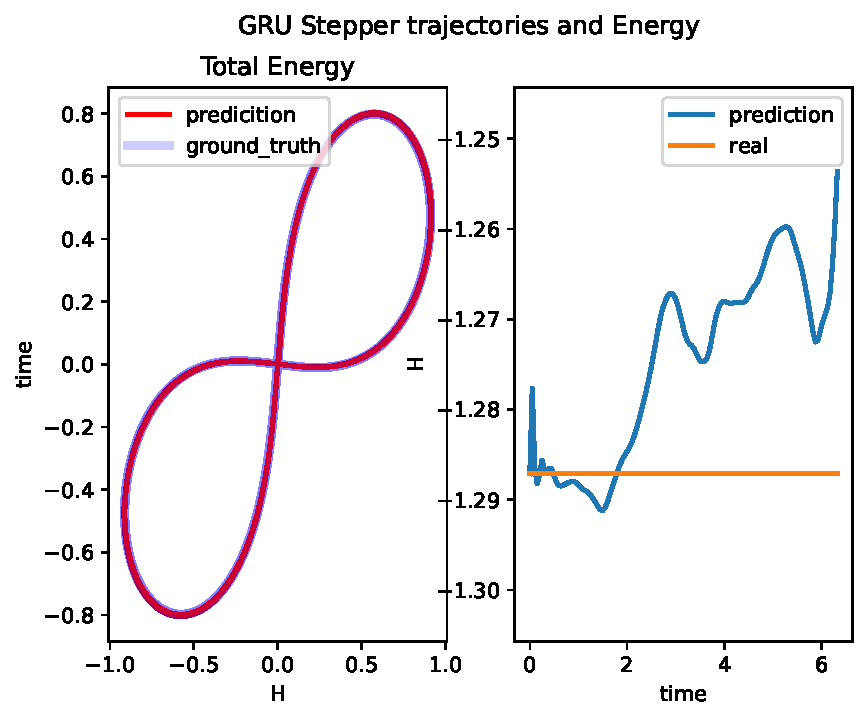
\includegraphics[width=\textwidth]{chapters/chapter5/body3_gre_traj.pdf}
		\caption{GRU Stepper}
	\end{subfigure}
	\hfill
	\begin{subfigure}[b]{0.3\textwidth}
		\centering
		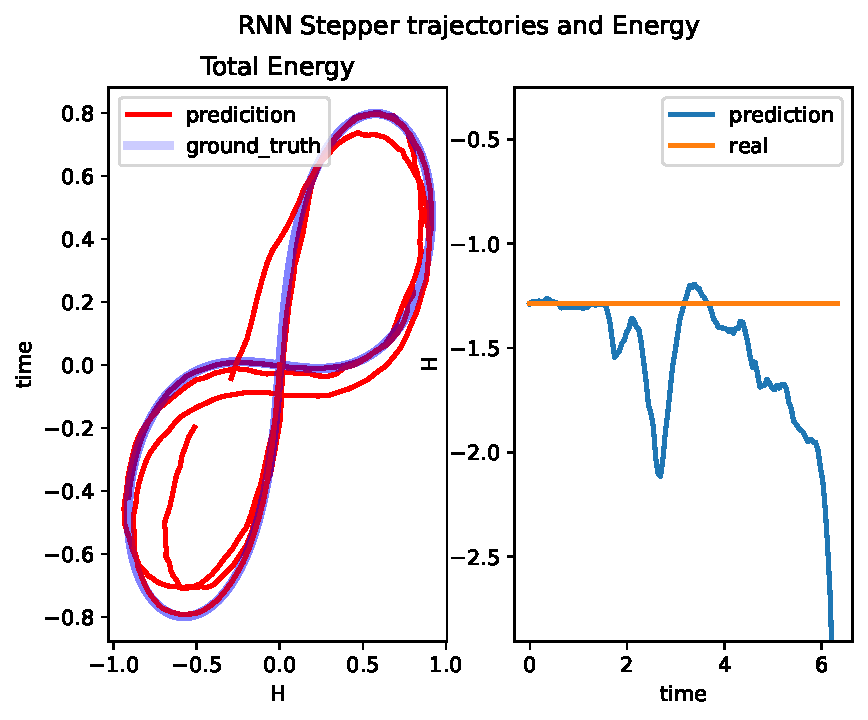
\includegraphics[width=\textwidth]{chapters/chapter5/body3_rne_traj.pdf}
		\caption{RNN stepper}
	\end{subfigure}
	
	\caption{Evaluation of the sample on the models, Trajectory and Energy(Threebody)}
	\label{body3_traj}
\end{figure}

\begin{figure}[H]
	\centering
	\begin{subfigure}[b]{0.3\textwidth}
		\centering
		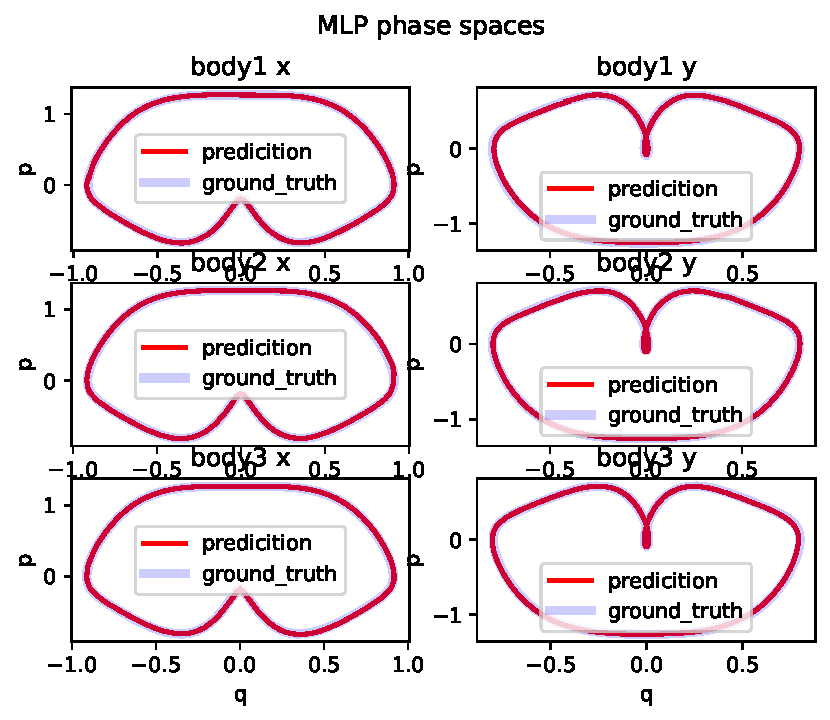
\includegraphics[width=\textwidth]{chapters/chapter5/body3_mlp_ps.pdf}
		\caption{MLP}
	\end{subfigure}
	\hfill
	\begin{subfigure}[b]{0.3\textwidth}
		\centering
		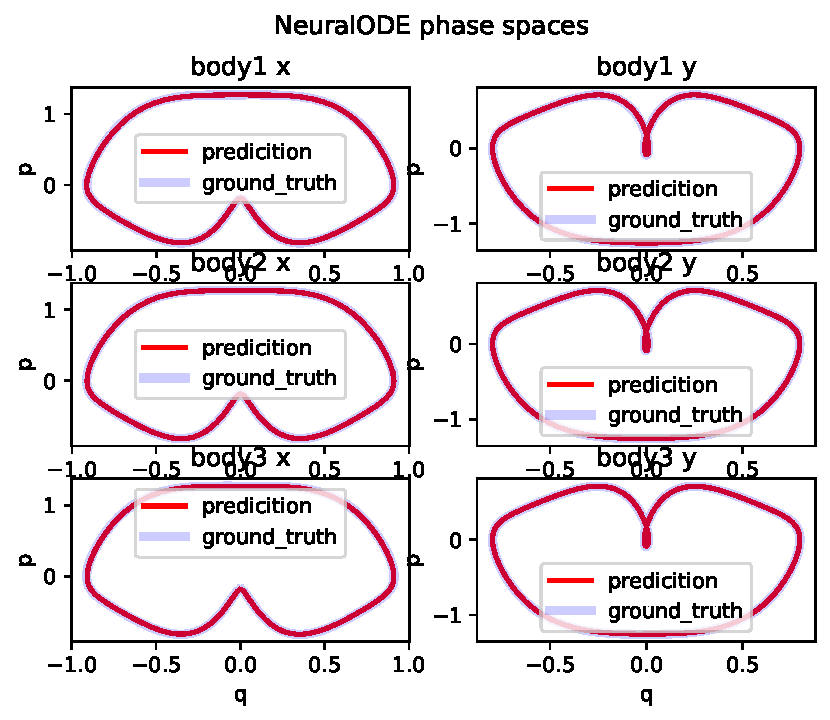
\includegraphics[width=\textwidth]{chapters/chapter5/body3_ode_ps.pdf}
		\caption{ODE}
	\end{subfigure}
	\hfill
	\begin{subfigure}[b]{0.3\textwidth}
		\centering
		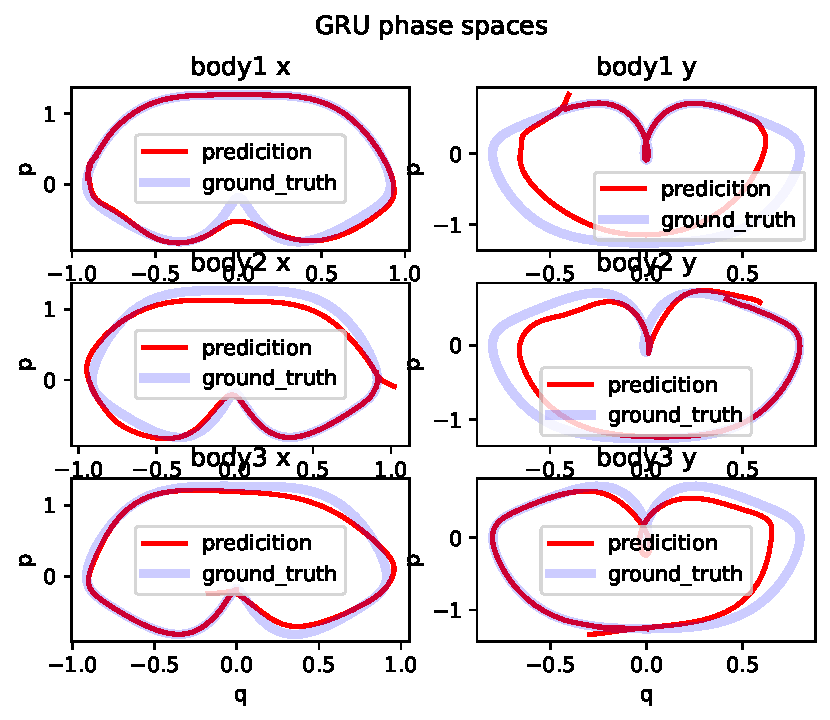
\includegraphics[width=\textwidth]{chapters/chapter5/body3_gru_ps.pdf}
		\caption{GRU}
	\end{subfigure}
	
	\vspace{0.5cm} % Adds vertical space between rows
	
	\begin{subfigure}[b]{0.3\textwidth}
		\centering
		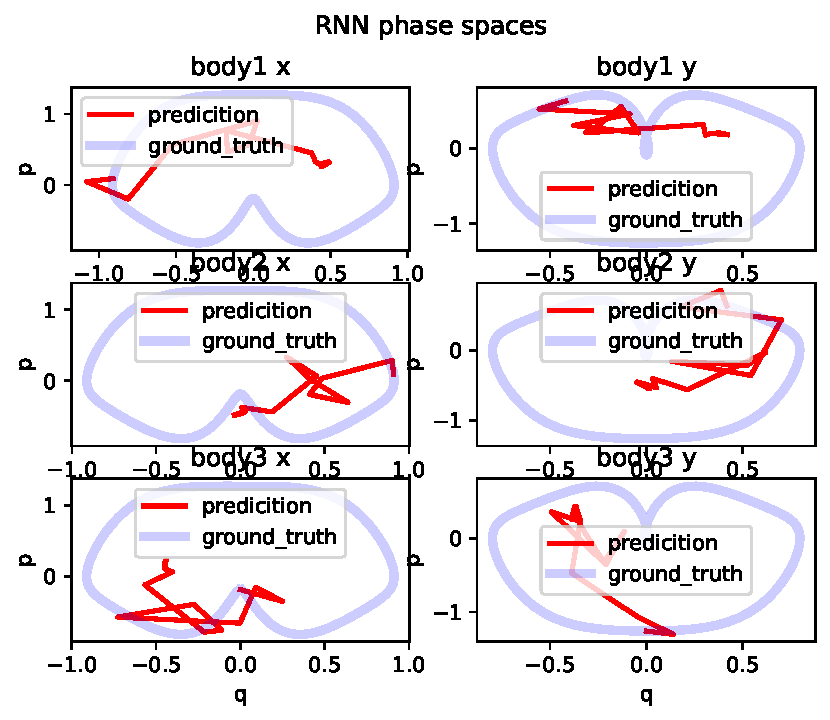
\includegraphics[width=\textwidth]{chapters/chapter5/body3_rnn_ps.pdf}
		\caption{RNN}
	\end{subfigure}
	\hfill
	\begin{subfigure}[b]{0.3\textwidth}
		\centering
		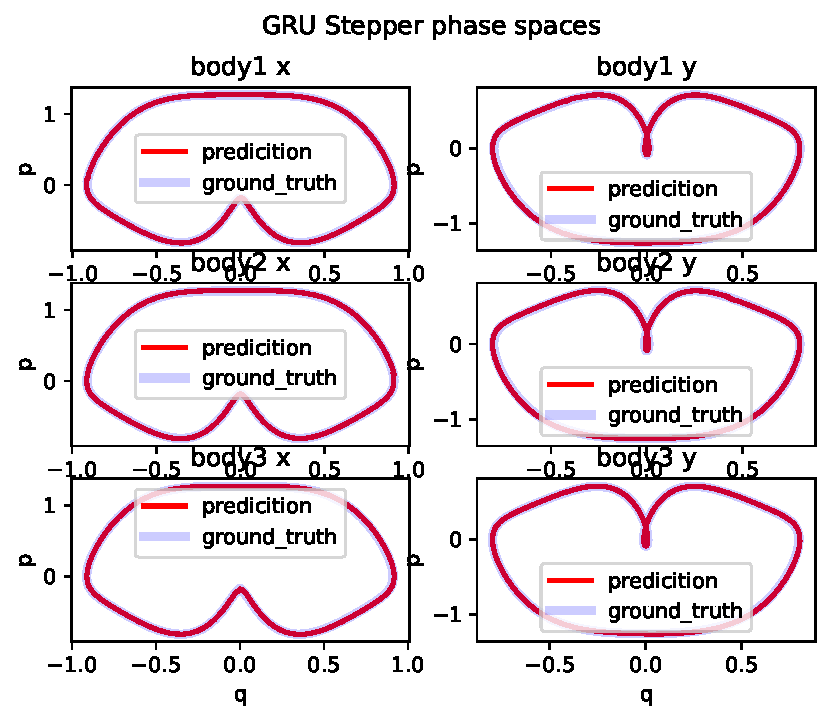
\includegraphics[width=\textwidth]{chapters/chapter5/body3_gre_ps.pdf}
		\caption{GRU Stepper}
	\end{subfigure}
	\hfill
	\begin{subfigure}[b]{0.3\textwidth}
		\centering
		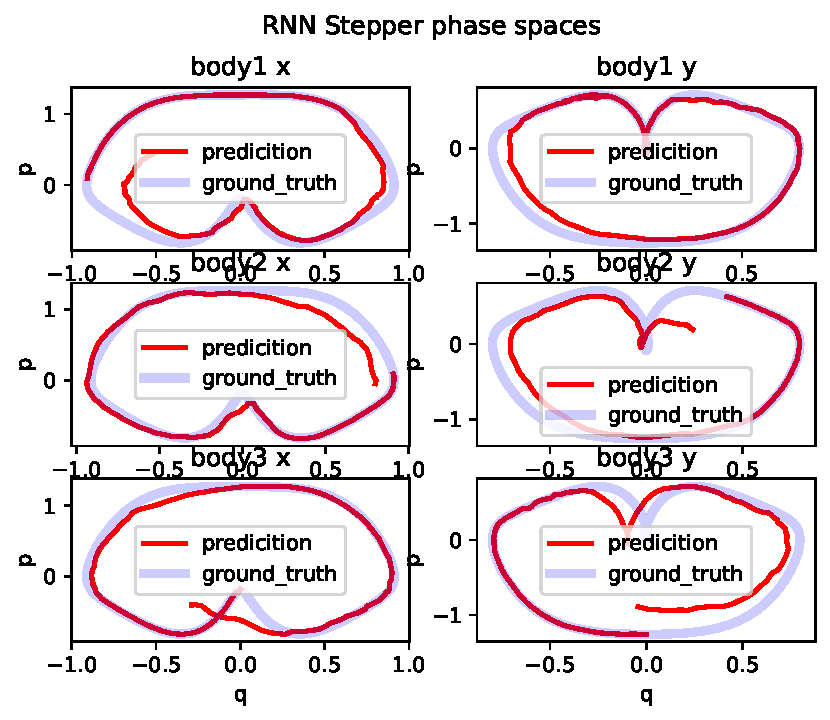
\includegraphics[width=\textwidth]{chapters/chapter5/body3_rne_ps.pdf}
		\caption{RNN stepper}
	\end{subfigure}
	
	\caption{Evaluation of the sample on the models, phase space (Threebody)}
	\label{body3_ps}
\end{figure} 




\section{Experimentation of Physics informed datasets on three body Dataset}
After the showcase of our datasets and architectures, we will now do some training of the physics informed neural networks. We choose two datasets, one will three body problem identical to the experiment before and one dataset with mixed solutions of the three body problems. We chosed carefully similar trajectories for better training performance. 
the models are:
\begin{itemize}
	\item improved Graph Hamiltonian Neural Network
	\item Hamiltonian Neural Network
	\item GRU- Graph Hamiltonian Neural Network(GAT layer)
\end{itemize}
This models are called physics informed not only because they are made through differentiation but all of the models gives Total energy from the model directly. With this information we can make physics-informed loss. 
The physics informed-loss that we chose is
\begin{equation}
	Loss =  \omega_rMSE(\dot{\mathbf{q}},\frac{d}{dt}\hat{\mathbf{q}}) + \omega_v MSE(\dot{\mathbf{p}},\frac{d}{dt}\hat{\mathbf{p}}) +
	\omega_h MSE(H(\mathbf{q},\mathbf{p}),\hat{H}) 
\end{equation} with $[\omega_r,\omega_v,\omega_h] =1.0,1.0,0.05$.

Hyperparameters of our models:
\begin{itemize}
	\item HNN\\ 
	2 layers with tanH activation after the first layer, \\
	hidden size: 256
	\item improved GHNN\\ 
	2 Combined(GAT + GCN) layers with tanH activation with dropout at attention $p=0.65$\\
	hidden size: 256\\
	output size before constructing H: 16
	\item GRUGHNN\\ 
	GRUcell + 2 GAT layers with tanH activation with dropout at attention $p=0.65$\\
	hidden size: 256\\
	output size before constructing H: 16
\end{itemize}
We trained our models for 200 epochs.
\subsection{Threebody dataset}
For this experiment we choosed 10 trajectories in domain $\alpha= \pi/8$. $\alpha$
is maximal angle which creates rotational region for creation of the dataset. From those 10 trajectories we made batches for training data and test data. The time sequence is 32 timepoints and 32 samples pro batch. The is $dt$=0.05.
After 100 epochs we get following results which can be observed in Figures \ref{div_traj} \ref{div_loss}.
\begin{figure}[H]
	\centering
	\begin{subfigure}[b]{0.3\textwidth}
		\centering
		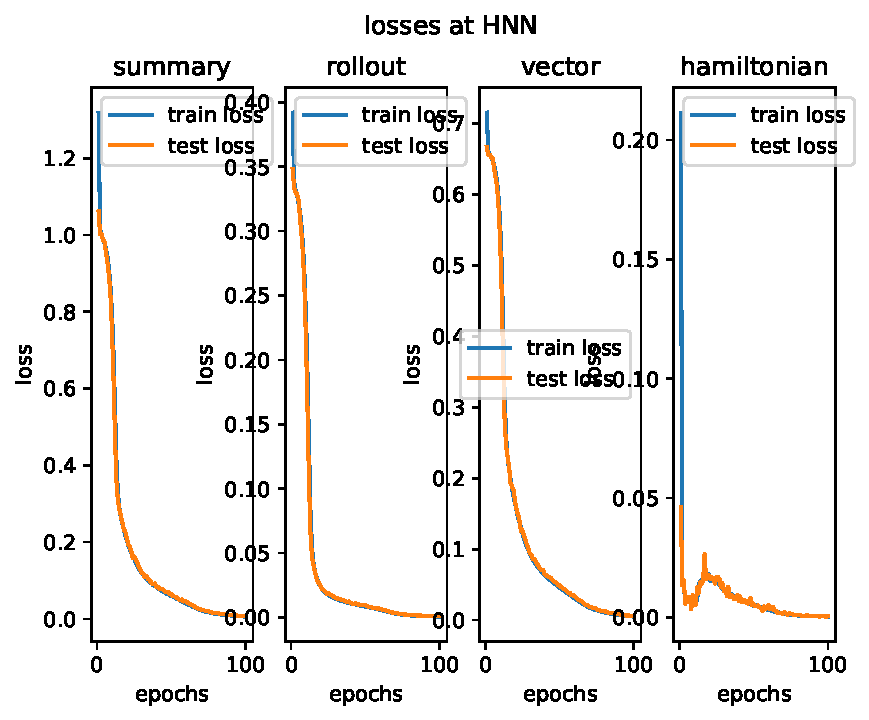
\includegraphics[width=\textwidth]{chapters/chapter5/figonly_hnn_loss.pdf}
		\caption{loss at HNN}
		\label{fig:image1}
	\end{subfigure}
	\hfill
	\begin{subfigure}[b]{0.3\textwidth}
		\centering
		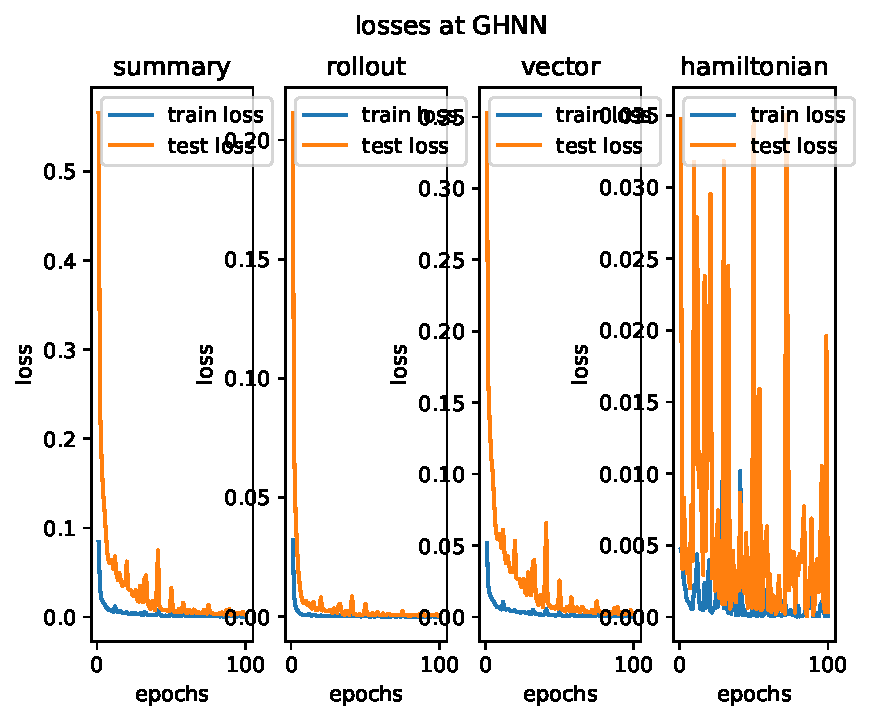
\includegraphics[width=\textwidth]{chapters/chapter5/figonly_ghnn_loss.pdf}
		\caption{loss at GHNN}
		\label{fig:image2}
	\end{subfigure}
	\hfill
	\begin{subfigure}[b]{0.3\textwidth}
		\centering
		\includegraphics[width=\textwidth]{chapters/chapter5/figonly_grughnn_loss.pdf}
		\caption{Loss at GRUGHNN}
		\label{fig:image3}
	\end{subfigure}
	
	\caption{Losses at various pinn models (threebody dataset)}
	\label{div_loss}
\end{figure}

% Second main plot with 3 subplots (horizontally aligned)
\begin{figure}[H]
	\centering
	\begin{subfigure}[b]{0.3\textwidth}
		\centering
		\includegraphics[width=\textwidth]{chapters/chapter5/figonly_hnn_traj.pdf}
		\caption{trajectories,phase spaces and H at HNN}
		\label{fig:image4}
	\end{subfigure}
	\hfill
	\begin{subfigure}[b]{0.3\textwidth}
		\centering
		\includegraphics[width=\textwidth]{chapters/chapter5/figonly_ghnn_traj.pdf}
		\caption{trajectories,phase spaces and H at GHNN}
		\label{fig:image5}
	\end{subfigure}
	\hfill
	\begin{subfigure}[b]{0.3\textwidth}
		\centering
		\includegraphics[width=\textwidth]{chapters/chapter5/figonly_grughnn_traj.pdf}
		\caption{trajectories,phase spaces and H at GRUGHNN}
		\label{fig:image6}
	\end{subfigure}
	
	\caption{Trajectories , phase spaces and hamiltonian at various pinn models}
	\label{div_traj}
\end{figure}

We can observe that hamiltonian at HNN and GHNN model is overall constant. Best performance shows the GRUGHNN where we have almost perfect trajectory with oscilating hamiltonian.

\begin{comment}

\subsection{Diverse solutions}
In this Dataset we took 5 unique diverse solutions of threebody problem. We used Figure 8\ref{diverse} as evaluation sample. First we set the time step to be $dt = 0.1$. With this information we got training and test set which is made from phase spaces on corresponding coordinates and hamiltonian value which is for every trajectory conserved. Every trajectory in the samples begins from the same coordinates under diverse moments/speeds.  

\begin{table}[H]
	\centering
	\begin{tabular}{ | c | m{5cm}| }
		\hline
		  & Specifications\\ 
		\begin{minipage}{.3\textwidth}
			\includegraphics[width=30mm, height=30mm]{chapters/chapter5/yarn}
		\end{minipage}
		&
		%\begin{minipage}[t]{5cm}
		\begin{itemize}
			\item Name : Yarn
			\item H: -1.196537
			\item T: 55.501762s
		\end{itemize}\\
		%\end{minipage}
		\hline
		  & Specifications\\ 
		\begin{minipage}{.3\textwidth}
			\includegraphics[width=30mm, height=30mm]{chapters/chapter5/fig8}
		\end{minipage}
		&
		%\begin{minipage}[t]{5cm}
		\begin{itemize}
			\item Name : Figure8
			\item H: -1.287146
			\item T: 6.324449s
		\end{itemize}\\
		%\end{minipage}
		\hline
		& Specifications\\ 
		\begin{minipage}{.3\textwidth}
			\includegraphics[width=30mm, height=30mm]{chapters/chapter5/moth}
		\end{minipage}
		&
		%\begin{minipage}[t]{5cm}
		\begin{itemize}
			\item Name : Moth
			\item H: -1.305861
			\item T: 28.670278s
		\end{itemize}\\
		%\end{minipage}
		\hline
		& Specifications\\ 
		\begin{minipage}{.3\textwidth}
			\includegraphics[width=30mm, height=30mm]{chapters/chapter5/v810}
		\end{minipage}
		&
		%\begin{minipage}[t]{5cm}
		\begin{itemize}
			\item Name : VIII 10
			\item H: -1.693544
			\item T: 48.894527s
		\end{itemize}\\
		%\end{minipage}
		\hline
		& Specifications\\ 
		\begin{minipage}{.3\textwidth}
			\includegraphics[width=30mm, height=30mm]{chapters/chapter5/googles}
		\end{minipage}
		&
		%\begin{minipage}[t]{5cm}
		\begin{itemize}
			\item Name : Googles
			\item H: -2.430116
			\item T: 10.466818s
		\end{itemize}\\
		%\end{minipage}
		\hline
	\end{tabular}
	\caption{diverse Dataset samples\cite{web}}
	\label{diverse}
\end{table}


For the models we get following plots\ref{div_loss}\ref{div_traj}
% First main plot with 3 subplots (horizontally aligned)

In those Figures we see that only GRUGHNN shows potential in training. In our evaluation trajectory plots we introduced figure 8 trajectory which wasn't in the dataset as a training sample. We know and assumpt that the trajectories won't be good or perfect. The point of this experiment was to see if those experiments are capable to make trajectories with somehow constant hamiltonian. As we see from trajectory figures our baseline achieves a constant hamiltonian value but not equal to true hamiltonian and GRUGHNN shows potential doing the same and the movement is more exaggerated but hamiliation tries to be conserved around the true value. Those models were trained for 300 epochs which equals to 1.5 days.    
\end{comment}
\subsection{Figure 8 solutions}
In this Dataset we use 4 Types of Figure 8 solutions which differs from eachother in period and energy. Those samples are in the table \ref{fig8} We use v.7.a, v.7.b, v.7.d solutions for training and testing and figure 8 for evaluation and visualization. We took 5 trajectories from every solution and it is fully supervised with loss mentioned before. Because of different periods, which results with different number of time points, we implemented stride and took every forth snapshot from the trajectories. For batching our time sequences have 32 timepoints and there are 32 samples pro batch. \\
In figures \ref{fig_loss}, \ref{fig_traj}, we can see their loss progression, trajectories and phase spaces.

\begin{table}[H]
	\centering
	\begin{tabular}{ | c | m{5cm}| }
		\hline
		& Specifications\\ 
		\begin{minipage}{.3\textwidth}
			\includegraphics[width=30mm, height=30mm]{chapters/chapter5/v1a}
		\end{minipage}
		&
		%\begin{minipage}[t]{5cm}
		\begin{itemize}
			\item Name : v1 a/ Figure 8
			\item H: -1.287146 
			\item T: 6.324449s
		\end{itemize}\\
		%\end{minipage}
		\hline
		& Specifications\\ 
		\begin{minipage}{.3\textwidth}
			\includegraphics[width=30mm, height=30mm]{chapters/chapter5/v7a}
		\end{minipage}
		&
		%\begin{minipage}[t]{5cm}
		\begin{itemize}
			\item Name : v.7.a 
			\item H: -1.570451 
			\item T: 32.849071s
		\end{itemize}\\
		%\end{minipage}
		\hline
		& Specifications\\ 
		\begin{minipage}{.3\textwidth}
			\includegraphics[width=30mm, height=30mm]{chapters/chapter5/v7c.pdf}
		\end{minipage}
		&
		%\begin{minipage}[t]{5cm}
		\begin{itemize}
			\item Name : v.7.c
			\item H: -1.504302
			\item T: 35.043086s
		\end{itemize}\\
		%\end{minipage}
		\hline
		& Specifications\\ 
		\begin{minipage}{.3\textwidth}
			\includegraphics[width=30mm, height=30mm]{chapters/chapter5/v7d.pdf}
		\end{minipage}
		&
		%\begin{minipage}[t]{5cm}
		\begin{itemize}
			\item Name : v.7.d
			\item H: -1.080763
			\item T: 57.545253s
		\end{itemize}\\
		%\end{minipage}
		\hline
	\end{tabular}
	\caption{Figure 8 Dataset samples\cite{web}}\label{diverse}
	\label{fig8}
\end{table}


% First main plot with 3 subplots (horizontally aligned)
\begin{figure}[H]
	\centering
	\begin{subfigure}[b]{0.3\textwidth}
		\centering
		\includegraphics[width=\textwidth]{chapters/chapter5/fignew_hnn_loss.pdf}
		\caption{loss at HNN}
		%\label{fig:image1}
	\end{subfigure}
	\hfill
	\begin{subfigure}[b]{0.3\textwidth}
		\centering
		\includegraphics[width=\textwidth]{chapters/chapter5/fignew_ghnn_loss.pdf}
		\caption{loss at GHNN}
	%	\label{fig:image2}
	\end{subfigure}
	\hfill
	\begin{subfigure}[b]{0.3\textwidth}
		\centering
		\includegraphics[width=\textwidth]{chapters/chapter5/fignew_grughnn_loss.pdf}
		\caption{Loss at GRUGHNN}
	%	\label{fig:image3}
	\end{subfigure}
	
	\caption{Losses at various models (figure dataset)}
	\label{fig_loss}
\end{figure}

% Second main plot with 3 subplots (horizontally aligned)
\begin{figure}[H]
	\centering
	\begin{subfigure}[b]{0.3\textwidth}
		\centering
		\includegraphics[width=\textwidth]{chapters/chapter5/fignew_hnn_traj.pdf}
		\caption{trajectories,phase spaces and H at HNN}
		%\label{fig:image4}
	\end{subfigure}
	\hfill
	\begin{subfigure}[b]{0.3\textwidth}
		\centering
		\includegraphics[width=\textwidth]{chapters/chapter5/fignew_ghnn_traj.pdf}
		\caption{trajectories,phase spaces and H at GHNN}
		%\label{fig:image5}
	\end{subfigure}
	\hfill
	\begin{subfigure}[b]{0.3\textwidth}
		\centering
		\includegraphics[width=\textwidth]{chapters/chapter5/fignew_gru_ghnn_traj.pdf}
		\caption{trajectories,phase spaces and H at GRUGHNN}
		%\label{fig:image6}
	\end{subfigure}
	
	\caption{Trajectories , phase spaces and hamiltonian at various models(figure dataset)}
	\label{fig_traj}
\end{figure}
We can clearly see that the proposed models are better then baseline HNN. They show better performance and better data fitting. Interestingly the hamiltonian on HNN and improved GHNN is almost constant and the trajectories have movement. Even though the trajectories of GRUGHNN are not accurate and hamiltonian tries to be conservative, it tries to follow the ground truth trajectory better then other models.  



\section{Experimentation of Physics informed models on N body problem and N pendelum}
In this experiment we took only physics informed graph models GHNN and GRUGHNN. Here we have two samples of datasets for n-pendelum and n body problem. The goal of this experiment is to see if the model is capable to generalize or make correct trajectory adding or discarding one more degree of freedom. For graph neural network that shouldn't be a problem because the size of the network depends not at size of the graph but on the size of the feature space. HNN model in this case is not usable.

We will use simmilar hyperparameters for our models for both cases:
\begin{itemize}
	\item GHNN\\ 
	2 GAT layers with tanH activation with dropout at attention $p=0.65$\\
	hidden size: 128\\
	output size before constructing H: 16
	\item GRUGHNN\\ 
	GRUcell + 2 GAT layers with tanH activation with dropout at attention $p=0.65$\\
	hidden size: 128\\
	output size before constructing H: 16
\end{itemize}

\subsection{N-body pendulum}
In this case we took 20 trajectories with 128 timepoints. The dataset is created with randomised inital values: $p_{\Theta} = 0$ and $\Theta =[-\pi,\pi]$ but we discarded those which trajectory is $|\Theta|>2\pi$. We batched training data with batch size of 32 with 32 points in trajectory, vectorfield and hamiltonian energy. We supervised within the loss
\begin{equation}
	Loss =  \omega_r(Hub({\mathbf{q}},\hat{\mathbf{q}}) + Hub({\mathbf{p}},\hat{\mathbf{p}})) +
	\omega_v(Hub(\dot{\mathbf{q}},\frac{d}{dt}\hat{\mathbf{q}}) + Hub(\dot{\mathbf{p}},\frac{d}{dt}\hat{\mathbf{p}})) +
	\omega_h Hub(H(\mathbf{q},\mathbf{p}),\hat{H}) 
\end{equation} with $\omega ={1.00,0.5,0.1}$.
\begin{table}[h!]
	\centering
	\caption{Evaluation of 3dof sample on various models and training procedures} % Add your caption here
	\label{tab:my_label}               % Add your label here
	\begin{tabular}{|l|l|l|l|}
		\hline
		dof3 & roll & vec & h\\ 
		\hline
		HGNN 3dof & 8.58 & 22.91 & 0.57 \\  
		\hline
		HGNN 4dof & 150.74 & 501.93 & 10.93 \\  
		\hline
		GRUHGNN 3dof & 2.57 & 21,7211 & 6,7363 \\  
		\hline
		GRUHGNN 4dof & 5.6 & 29.85 & 5.96 \\  
		\hline
	\end{tabular}
\end{table}
\begin{table}[h!]
	\centering
	\caption{Evaluation of 4dof sample on various models and training procedures} % Add your caption here
	\label{tab:my_label}               % Add your label here
	\begin{tabular}{|l|l|l|l|}
		\hline
		dof4 & roll & vec & h\\ 
		\hline
		HGNN 3dof & 12.35 & 31.85 & 2.12 \\  
		\hline
		HGNN 4dof & 10.45 & 32.28 & 22.9 \\  
		\hline
		GRUHGNN 3dof & 5.61 & 24.72 & 10.71 \\  
		\hline
		GRUHGNN 4dof & 7.00 & 33.1747 & 12.5609 \\  
		\hline
	\end{tabular}
\end{table}






\begin{figure}[H]
	\centering
	\begin{subfigure}[b]{0.4\textwidth}
		\centering
		\includegraphics[width=\textwidth]{chapters/chapter5/loss_3dof.pdf}
		\caption{Losses at 3dof training}
		%\label{fig:image4}
	\end{subfigure}
	\hfill
	\begin{subfigure}[b]{0.4\textwidth}
		\centering
		\includegraphics[width=\textwidth]{chapters/chapter5/loss_4dof.pdf}
		\caption{Losses at 4dof training}
		%\label{fig:image5}
	\end{subfigure}
	
	
	\caption{Losses till 500 epochs(Pendulum)}
	\label{fig_traj}
\end{figure}
\begin{table}[h!]
\centering
\caption{Evaluation of 3dof sample on GRUGNN and training procedures} % Add your caption here
\label{tab:pend500}               % Add your label here
\begin{tabular}{|l|l|l|l|l|}
	\hline
	dof3 & roll & vec & h\\ 
	\hline
	GRUHGNN 3dof & 3.49 & 23,17 & 7.7 \\  
	\hline
	GRUHGNN 4dof & 6.71 & 26.6007 & 45.09 \\  
	\hline
\end{tabular}
\end{table}



\begin{table}[h!]
\centering
\caption{Evaluation of 4dof sample on GRUGNN models and training procedures, } % Add your caption here
\label{tab:pend1000}               % Add your label here
\begin{tabular}{|l|l|l|l|l|}
	\hline
	dof4 & roll & vec & h\\  
	\hline
	GRUHGNN 3dof & 59.33 & 24.95 & 20.82 \\  
	\hline
	GRUHGNN 4dof & 8.47 & 26.8 & 50.2 \\  
	\hline
\end{tabular}
\end{table}

\begin{figure}[H]
	\centering
	\begin{subfigure}[b]{0.4\textwidth}
		\centering
		\includegraphics[width=\textwidth]{chapters/chapter5/loss_3dof1000.pdf}
		\caption{Losses at 3dof training}
		%\label{fig:image4}
	\end{subfigure}
	\hfill
	\begin{subfigure}[b]{0.4\textwidth}
		\centering
		\includegraphics[width=\textwidth]{chapters/chapter5/loss_4dof1000.pdf}
		\caption{Losses at 4dof training}
		%\label{fig:image5}
	\end{subfigure}
	
	
	\caption{Losses till 1000 epochs on GRUGHNN(Pendelum)}
	\label{fig_traj}
\end{figure}

\begin{figure}[htbp]
	\centering
	% First row of subplots
	\begin{subfigure}[b]{0.45\textwidth}
		\centering
		\includegraphics[width=\textwidth]{chapters/chapter5/traj_3dof3_pend.pdf} % Replace with your image file
		\caption{GRUGHNN trained on 3dof sample and made 3dof trajectory}
		\label{fig:sub1}
	\end{subfigure}
	\hfill
	\begin{subfigure}[b]{0.45\textwidth}
		\centering
		\includegraphics[width=\textwidth]{chapters/chapter5/traj_4dof3_pend.pdf} % Replace with your image file
		\caption{GRUGHNN trained on 4dof sample and made 3dof trajectory}
		\label{fig:sub2}
	\end{subfigure}
	
	% Second row of subplots
	\vspace{0.5cm}
	\begin{subfigure}[b]{0.45\textwidth}
		\centering
		\includegraphics[width=\textwidth]{chapters/chapter5/traj_3dof4_pend.pdf} % Replace with your image file
		\caption{GRUGHNN trained on 3dof sample and made 4dof trajectory}
		\label{fig:sub3}
	\end{subfigure}
	\hfill
	\begin{subfigure}[b]{0.45\textwidth}
		\centering
		\includegraphics[width=\textwidth]{chapters/chapter5/traj_4dof4_pend.pdf} % Replace with your image file
		\caption{GRUGHNN trained on 4dof sample and made 4dof trajectory}
		\label{fig:sub4}
	\end{subfigure}
	
	\caption{trajectories of pendelums after 1000 epochs}
	\label{pend_traj}
\end{figure}

In the tables \ref{tab:pend500} and  \ref{tab:pend1000} we compared the HuberLoss values of evaluation trajectory of 3dof pendulum and 4dof pendelum on the PINN models, which are train on 3dof and 4dof dataset under 500 epochs. For better comparison we evaluated  1000 epochs only on GRUGHNN. Chosed trajectories for visualization iare fully unknown to the models.\\ 
From the values in the tables\ref{tab:pend500} and \ref{tab:pend1000} we can read that GHNN dosen't like losing degree of freedom. We see very big difference in those values. In other cases there is difference but not exaggerated.\\
Interestingly Huberloss for the vector field at GRUGHNN is realtivly stable in comparison with GHNN.  
The trajectories are observable in figure \ref{pend_traj}

\subsection{N-body problem}
In the similar manner as N-pendelum we made N-body Problem.
First we needed to set up domain of movement and we chosed 20 samples of trajectories of 128 timesteps with $dt =0.01$. In the dataset we have position velocity and energy and it is suprivised same as N-pendelum case and we reused only GRUGHNN model because it showed greatest performance in last experiments. Training was done trough 1000 epochs. This is just proof of concept that adding and discarding the graph nodes is possible.
\begin{table}[h!]
	\centering
	\caption{Evaluation of 3dof sample on GRUGNN and training procedures, (Nbody)} % Add your caption here
	\label{nbody_9dof}  
\begin{tabular}{|l|l|l|l|l|}
	\hline
	dof3 & roll & vec & h\\  
	\hline
	GRUHGNN 3dof & 0.88 & 9.19 & 6.03 \\  
	\hline
	GRUHGNN 4dof & 0.87 & 6.97 & 5.81 \\  
	\hline
\end{tabular}
\end{table}

\begin{table}[h!]
	\centering
	\caption{Evaluation of 4dof sample on GRUGNN and training procedures (Nbody)} % Add your caption here
	\label{nbody_10dof}  
\begin{tabular}{|l|l|l|l|l|}
	\hline
	dof4 & roll & vec & h\\  
	\hline
	GRUHGNN 3dof & 1.25 & 7.39 & 9.37 \\  
	\hline
	GRUHGNN 4dof & 1.08 & 10.11 & 9.37 \\  
	\hline
\end{tabular}
\end{table}



\begin{figure}[H]
	\centering
	\begin{subfigure}[b]{0.4\textwidth}
		\centering
		\includegraphics[width=\textwidth]{chapters/chapter5/loss_9.pdf}
		\caption{Losses at 9 bodies training}
		%\label{fig:image4}
	\end{subfigure}
	\hfill
	\begin{subfigure}[b]{0.4\textwidth}
		\centering
		\includegraphics[width=\textwidth]{chapters/chapter5/loss_10.pdf}
		\caption{Losses at 10 bodies training}
		%\label{fig:image5}
	\end{subfigure}
	
	
	\caption{Losses till 1000 epochs on GRUGHNN (Nbody)}
	\label{fig_traj}
\end{figure}

\begin{figure}[htbp]
	\centering
	% First row of subplots
	\begin{subfigure}[b]{0.45\textwidth}
		\centering
		\includegraphics[width=\textwidth]{chapters/chapter5/traj_9dof_9.pdf} % Replace with your image file
		\caption{GRUGHNN trained on 9dof sample and made 9dof trajectory}
		\label{fig:sub1}
	\end{subfigure}
	\hfill
	\begin{subfigure}[b]{0.45\textwidth}
		\centering
		\includegraphics[width=\textwidth]{chapters/chapter5/traj_10dof_9.pdf} % Replace with your image file
		\caption{GRUGHNN trained on 10dof sample and made 9dof trajectory}
		\label{fig:sub2}
	\end{subfigure}
	
	% Second row of subplots
	\vspace{0.5cm}
	\begin{subfigure}[b]{0.45\textwidth}
		\centering
		\includegraphics[width=\textwidth]{chapters/chapter5/traj_9dof_10.pdf} % Replace with your image file
		\caption{GRUGHNN trained on 9dof sample and made 10dof trajectory}
		\label{fig:sub3}
	\end{subfigure}
	\hfill
	\begin{subfigure}[b]{0.45\textwidth}
		\centering
		\includegraphics[width=\textwidth]{chapters/chapter5/traj_10dof_10.pdf} % Replace with your image file
		\caption{GRUGHNN trained on 10dof sample and made 10dof trajectory}
		\label{fig:sub4}
	\end{subfigure}
	\caption{Trajectories of nbody after 1000 epochs}
	\label{fig:body_Traj}
\end{figure}

\begin{figure}[htbp]
	\centering
	\includegraphics[width=0.8\textwidth]{chapters/chapter5/nbody_hamiltonian.pdf} % Replace with the path to your image file
	\caption{Hamiltonian of nbody cases}
	\label{nbody_ham}
\end{figure}

The results of the adding and discarding a body are really suprising good enough. The HuberLoss in the tables \ref{nbody_9dof} and \ref{nbody_10dof} shows relatively simmilar values Still the model tolerates more losing the body then gain it. This can be observed in \ref{body_traj} It is fully understandable looking at Nbody problem. Adding a body we could heavy disrupt the system.
Mostly interesting result is hamiltonian figure \ref{nbody_ham}. It shows that model trained on 9dof sample better accepts 10dof sample. Following the logic it is possible because we used GAT layers which at training of 4dof samples had few more weighting factors to create and fit. \\
With those experiments we got an good insight in the capabilities in those PINN models.